\documentclass[11pt]{article}

\usepackage[utf8]{inputenc}
\usepackage[T1]{fontenc}
\usepackage[spanish,es-tabla]{babel}
\usepackage[margin=2.5cm]{geometry}
\usepackage{amsmath}
\usepackage{booktabs}
\usepackage{longtable}
\usepackage{graphicx}
\usepackage{hyperref}

\title{Competencia espacial y traspaso de precios en el mercado chileno de combustibles\\[4pt]
\large Reporte técnico}
\author{Joaquín Martínez Ojeda}
\date{\today}

\begin{document}

\maketitle

\section{Datos}
\label{sec:datos}

La base final es un panel no balanceado de reportes de precios minoristas de
combustibles en Chile, a nivel de estación de servicio por combustible y
fecha de reporte, enriquecido con precios mayoristas semanales, atributos de
las estaciones y medidas de competencia espacial construidas a partir de la
geolocalización de cada estación. Cubre desde el 1 de enero de 2012 hasta el
12 de julio de 2026 y contiene 4.603.798 observaciones sobre 2.086
estaciones, cuatro combustibles (gasolinas de 93, 95 y 97 octanos y diésel),
146 distribuidores y las 16 regiones del país.

\subsection{Fuentes}
\label{sec:fuentes}

La base combina tres fuentes.

\begin{enumerate}
  \item \textbf{Precios minoristas (CNE).} Reportes de precios por estación y
  combustible publicados por la Comisión Nacional de Energía. La fuente cambia
  de estructura en 2023. Existe un formato antiguo (2012 a 2022, sin hora de
  reporte) y un formato vigente (2023 en adelante, con hora de reporte,
  modalidad de atención e indicadores de electrolineras). Ambos formatos se
  armonizan a un esquema común (Sección~\ref{sec:limpieza}).
  \item \textbf{Atributos de estaciones (CNE).} Tabla transversal con medios de
  pago aceptados y servicios ofrecidos (baño público, tienda de conveniencia,
  lavado de autos, entre otros) por estación, además de códigos
  administrativos de región y comuna. Los atributos se toman de la última
  actualización reportada por cada estación y se tratan como constantes en el
  tiempo.
  \item \textbf{Precios mayoristas (MEPCO).} Serie semanal de precios de
  paridad de importación con y sin el ajuste del Mecanismo de Estabilización de
  Precios de los Combustibles (MEPCO), junto con el componente variable del
  impuesto específico (UTM/m$^3$), para gasolina 93, gasolina 97 y diésel. La
  serie no cubre la gasolina 95, por lo que las variables mayoristas quedan
  sin valor para ese combustible.
\end{enumerate}

\subsection{Limpieza y armonización}
\label{sec:limpieza}

Los códigos de estación se normalizan y los nombres de distribuidor, comuna y
región se homologan a etiquetas canónicas entre ambos formatos de la CNE. Las
marcas Petrobras y Aramco se unifican en una sola etiqueta por tratarse de la
misma red tras el cambio de propiedad.

Los precios se depuran con una regla de tres pasos que recodifica como
faltantes los valores centinela, corrige errores de dígitos extra contra la
mediana anual del combustible y descarta precios inverosímiles.\footnote{Los
valores $0$ y $99.999.999$ se recodifican como faltantes. Si un precio supera
el doble de la mediana anual de su combustible, se divide por 10 o por 100
cuando el valor resultante queda dentro de $\pm 35\%$ de esa mediana, y se
recodifica como faltante en caso contrario. Los precios bajo \$200/L se
recodifican como faltantes. Las filas sin precio válido se eliminan.} A cada
estación se le asigna una única coordenada, la modal entre sus reportes, tras
validar que las coordenadas caigan en el rango factible para
Chile.\footnote{Se descartan latitudes positivas o menores a $-90^\circ$ y
longitudes positivas o menores a $-180^\circ$. Algunas estaciones fueron
re-geocodificadas levemente entre años, lo que motiva el uso de la coordenada
modal.}

En el formato vigente la CNE reporta por separado los precios de autoservicio
(grados con prefijo ``A''). Ambas modalidades se colapsan a un mismo grado de
combustible y la modalidad queda registrada en la variable
\texttt{service\_type}. El formato antiguo se usa hasta el 31 de diciembre de
2022 y el vigente desde el 1 de enero de 2023. Las variables que solo existen
en el formato vigente quedan como faltantes en el período antiguo.

La tabla de atributos cubre 1.739 de las 2.086 estaciones y se cruza con los
precios mediante un \emph{left join}, de modo que las estaciones sin
atributos (típicamente las que salieron del mercado antes del formato
vigente) conservan sus precios con atributos faltantes.\footnote{El archivo
de atributos provenía de una planilla corrompida por una ida y vuelta por
Excel. Era un CSV delimitado por punto y coma con decimales de coma, cuyas
filas fueron partidas en las comas decimales y parcialmente fusionadas. Se
reconstruyó programáticamente reuniendo las celdas, separando en saltos de
línea y conservando solo los registros bien formados de 37 campos.}

\subsection{Cruce con precios mayoristas}
\label{sec:mepco}

A cada reporte minorista se le asigna el precio mayorista vigente en su
fecha, es decir, la última cotización semanal del MEPCO en o antes de la
fecha del reporte (\emph{rolling join} hacia atrás). Se incluyen el precio de
paridad sin MEPCO, el precio con MEPCO y el componente variable del impuesto
específico. También se construye la primera diferencia de ambas series en
cada actualización semanal, que mide el tamaño del shock de costo que
enfrenta la estación cuando su precio mayorista vigente cambió por última
vez.

\subsection{Variables derivadas}
\label{sec:derivadas}

\paragraph{Ventana de actividad.} Para cada estación se registran la primera
y la última fecha en que aparece en los datos, que definen su ventana de
actividad y alimentan las medidas de competencia.

\paragraph{Tiempo de evento.} La base incluye el tiempo en días relativo al
shock del MEPCO del 26 de marzo de 2026 y un indicador de período posterior
al shock.

\paragraph{Rigidez de precios.} Dentro de cada par estación-combustible los
reportes se agrupan en tramos de precio constante. Se registra si el reporte
es un punto de cambio y los días transcurridos desde el último cambio. El
primer tramo observado de cada estación no tiene inicio conocido (censura por
la izquierda), por lo que ambas variables quedan indefinidas en la primera
fecha de cada estación.

\paragraph{Competencia espacial.} Las distancias entre las 2.086 estaciones
se calculan con la fórmula del haversine sobre la coordenada modal de cada
una. Para radios $r \in \{1,\dots,5\}$ km, \texttt{competitors\_rkm} cuenta
las estaciones rivales dentro del radio que estaban activas en la fecha del
reporte, es decir, cuya ventana de actividad contiene esa fecha. Se agrega
una medida continua de intensidad,

\begin{equation}
\label{eq:intensity}
\mathit{CI}_{it} \;=\; \sum_{j \neq i:\; d_{ij} \le 10\text{ km}}
\frac{\mathbf{1}\{j \text{ activa en } t\}}{\max(d_{ij},\, 0{,}1)},
\end{equation}

que pondera a cada rival por el inverso de su distancia dentro de un radio de
10 km.\footnote{El piso de 100 m evita que pares de coordenadas casi
duplicadas, probable ruido de geocodificación, dominen la medida.} En
promedio, una estación enfrenta 2,2 rivales activos dentro de 1 km y 22,8
dentro de 5 km.

\paragraph{Estructura de marca.} La etiqueta \emph{sin bandera} de la CNE
identifica estaciones sin marca. Entre los distribuidores con nombre, los que
operan una sola estación se tratan como operadores independientes y no como
redes. La variable \texttt{is\_franchise} marca a las estaciones de
distribuidores con marca y más de una estación. Bajo esta definición, el
95,1\% de las observaciones corresponde a estaciones de red.

\subsection{Unidad de observación y estructura del panel}
\label{sec:estructura}

La unidad de observación es el reporte de precio y una estación puede
reportar más de una vez por día. En el período antiguo, sin hora de reporte,
existen alrededor de 222 mil filas adicionales a nivel
estación-combustible-día por reportes intradiarios. En el período vigente los
reportes se distinguen por hora y por modalidad de atención. El panel es no
balanceado. Las estaciones entran y salen de la muestra y la frecuencia de
reporte varía entre estaciones y en el tiempo. Los agregados semanales usados
en el análisis se construyen aguas abajo a partir de esta base. La
Tabla~\ref{tab:diccionario} resume las variables de la base final.

\begin{longtable}{p{5.2cm} p{9.8cm}}
\caption{Diccionario de variables de la base final
(\texttt{data/processed/database.csv}).}
\label{tab:diccionario}\\
\toprule
Variable & Descripción \\
\midrule
\endfirsthead
\toprule
Variable & Descripción \\
\midrule
\endhead
\bottomrule
\endfoot
\multicolumn{2}{l}{\emph{Identificación y ubicación}} \\
\texttt{id} & Código CNE de la estación. \\
\texttt{date}, \texttt{time} & Fecha y hora del reporte (hora solo desde 2023). \\
\texttt{fuel} & Combustible: \texttt{93}, \texttt{95}, \texttt{97}, \texttt{di} (diésel). \\
\texttt{distributor} & Distribuidor (marca) homologado. \\
\texttt{municipality}, \texttt{region} & Comuna y región (etiquetas canónicas). \\
\texttt{codigo\_region}, \texttt{codigo\_comuna} & Códigos administrativos oficiales. \\
\texttt{latitud}, \texttt{longitud} & Coordenada modal de la estación. \\
\addlinespace
\multicolumn{2}{l}{\emph{Precio minorista}} \\
\texttt{price} & Precio minorista (\$/L), depurado. \\
\texttt{service\_type} & Atendido o autoservicio (solo desde 2023). \\
\texttt{ev\_station}, \texttt{gas\_station} & Indicadores de electrolinera y de estación de combustible (solo desde 2023). \\
\addlinespace
\multicolumn{2}{l}{\emph{Precios mayoristas (MEPCO, sin cobertura para la 95)}} \\
\texttt{wholesale\_w\_o}, \texttt{wholesale\_w} & Precio de paridad vigente sin y con MEPCO (\$/L). \\
\texttt{variable\_specific\_tax\_utm\_m3} & Componente variable del impuesto específico (UTM/m$^3$). \\
\texttt{d\_wholesale\_w\_o}, \texttt{d\_wholesale\_w} & Cambio del precio mayorista en su última actualización. \\
\addlinespace
\multicolumn{2}{l}{\emph{Atributos de la estación (constantes, faltantes si la estación no está en la tabla de atributos)}} \\
\texttt{efectivo}, \texttt{tarjeta\_credito}, \texttt{tarjeta\_debito}, \texttt{app\_pago}, \texttt{billetera\_digital} & Medios de pago aceptados. \\
\texttt{cajero\_automatico}, \texttt{banio\_publico}, \texttt{farmacia}, \texttt{tienda\_conveniencia}, \texttt{compresor\_aire\_neumaticos}, \texttt{lavado\_auto}, \texttt{juegos\_infantiles}, \texttt{servicios\_mantencion}, \texttt{surtidor\_camiones}, \texttt{duchas}, \texttt{lubricentro} & Servicios ofrecidos. \\
\texttt{fecha\_actualizacion} & Fecha de la última actualización de atributos. \\
\addlinespace
\multicolumn{2}{l}{\emph{Panel, evento y rigidez}} \\
\texttt{first\_date}, \texttt{last\_date} & Ventana de actividad de la estación. \\
\texttt{days\_to\_event}, \texttt{post\_shock} & Tiempo de evento e indicador posterior al shock del 26/03/2026. \\
\texttt{price\_changed} & El reporte es un punto de cambio de precio (NA en la primera fecha de la estación). \\
\texttt{days\_since\_last\_price\_change} & Días desde el último cambio de precio (NA en la primera fecha). \\
\addlinespace
\multicolumn{2}{l}{\emph{Competencia espacial y estructura de marca}} \\
\texttt{competitors\_1km} a \texttt{competitors\_5km} & Número de rivales activos dentro de 1 a 5 km en la fecha del reporte. \\
\texttt{competition\_intensity} & Intensidad de competencia, ecuación~\eqref{eq:intensity}. \\
\texttt{distributor\_n\_stations} & Número de estaciones del distribuidor. \\
\texttt{is\_franchise} & Distribuidor con marca y más de una estación. \\
\end{longtable}

\section{Proyecciones locales sobre el historial de actualizaciones del MEPCO}
\label{sec:lp}

Esta sección estima cuánto y a qué velocidad el precio minorista responde a
los cambios del costo mayorista, mediante proyecciones locales
que usan como shocks las 622 actualizaciones semanales del MEPCO entre el 7
de agosto de 2014 y el 2 de julio de 2026, para las gasolinas 93 y 97 y el
diésel.\footnote{La gasolina 95 se excluye porque no tiene precio mayorista
de referencia en el MEPCO.} El coeficiente objetivo es la elasticidad
acumulada del precio al costo en cada horizonte, cuyo valor de referencia
bajo traspaso completo es 1.

\subsection{Especificación}
\label{sec:lp_especificacion}

La serie de precios de cada par estación-combustible se remuestrea sobre el
calendario semanal del MEPCO, de modo que el shock y la respuesta comparten
frecuencia.\footnote{El reporte minorista es irregular, por lo que en cada
fecha del calendario MEPCO se toma la última observación disponible del par,
dentro de su ventana de actividad. La grilla resultante tiene 3.238.217
observaciones semanales sobre 5.794 pares estación-combustible y 2.038
estaciones.} Para cada horizonte $h = 0, 1, \dots, 12$ semanas se estima por
MCO

\begin{equation}
\label{eq:lp}
\log p_{i,f,t+h} - \log p_{i,f,t-1}
= \alpha_{if}^{(h)}
+ \beta_h \, \Delta \log w_{f,t}
+ \sum_{\ell=1}^{L} \gamma_{\ell}^{(h)} \, \Delta \log w_{f,t-\ell}
+ \varepsilon_{i,f,t+h},
\end{equation}

donde $p_{i,f,t}$ es el precio minorista de la estación $i$ para el
combustible $f$ en la semana $t$, $w_{f,t}$ es el precio mayorista con MEPCO
y $\alpha_{if}^{(h)}$ es un efecto fijo estación por combustible. El
coeficiente $\beta_h$ es la elasticidad acumulada del precio al costo $h$
semanas después del shock. Los $L = 13$ rezagos del shock se incluyen porque
el MEPCO presenta correlación serial y, sin ellos, $\beta_h$ recogería
también la respuesta a shocks anteriores correlacionados.\footnote{La
autocorrelación de primer orden de $\Delta \log w$ es 0,17 para la gasolina
93. El orden $L$ se eligió ajustando un AR($p$) por AIC a la serie de cada
combustible con máximo 20 rezagos, lo que arrojó órdenes de 13, 12 y 12 para
93, 97 y diésel. Se usa el máximo.} Los errores estándar se agrupan por
estación en todas las especificaciones del reporte.\footnote{Las estimaciones
se realizaron en R con el paquete \texttt{fixest}.} La muestra de estimación
tiene 3.174.712 observaciones en $h = 0$ (5.777 pares estación-combustible,
2.035 estaciones) y 3.105.611 en $h = 12$.

La ecuación~\eqref{eq:lp} se reestima por submuestras en cinco dimensiones:
combustible, marca, terciles de competidores activos dentro de 2 km, un
indicador de estación de carretera y macrozona.\footnote{La marca es el
distribuidor modal de la estación en su historia, distinguiendo Copec, Shell
y Aramco-Petrobras del resto (independientes). Los cortes de los terciles se
calculan sobre la grilla remuestreada. Carretera se define como ofrecer
duchas o surtidor de camiones, amenidades propias de paradas de ruta. Las
macrozonas son norte (Arica a Coquimbo), centro (Valparaíso a Biobío) y sur
(Araucanía a Magallanes), porque varias regiones extremas tienen muy pocas
estaciones para una estimación propia.} Como el efecto fijo ya absorbe toda
característica invariante de la estación, estos cortes no son controles
contra confusión sino la pregunta de si la elasticidad misma difiere entre
grupos.

\subsection{Resultados}
\label{sec:lp_resultados}

La Tabla~\ref{tab:lp_pooled} presenta la trayectoria agregada y por
combustible y la Tabla~\ref{tab:lp_het} los cortes de heterogeneidad. Las
Figuras~\ref{fig:lp_fuel} a~\ref{fig:lp_carretera_macro} muestran las
trayectorias completas con bandas de confianza al 95\%.

\begin{table}[htbp]
\centering
\caption{Proyecciones locales: traspaso acumulado del costo mayorista al
precio minorista, agregado y por combustible.}
\label{tab:lp_pooled}
\begin{tabular}{lccccc}
\toprule
 & \multicolumn{5}{c}{Horizonte $h$ (semanas)} \\
\cmidrule(lr){2-6}
 & 0 & 2 & 4 & 8 & 12 \\
\midrule
Agregado          & 0,565 & 0,732 & 0,882 & 1,017 & 0,922 \\
                  & (0,007) & (0,008) & (0,010) & (0,011) & (0,009) \\
\addlinespace
Gasolina 93       & 0,593 & 0,793 & 0,957 & 1,165 & 1,103 \\
                  & (0,007) & (0,008) & (0,010) & (0,012) & (0,011) \\
Gasolina 97       & 0,585 & 0,762 & 0,909 & 1,119 & 1,080 \\
                  & (0,007) & (0,009) & (0,010) & (0,012) & (0,011) \\
Diésel            & 0,549 & 0,700 & 0,842 & 0,928 & 0,815 \\
                  & (0,007) & (0,008) & (0,010) & (0,011) & (0,009) \\
\bottomrule
\end{tabular}

\medskip
\begin{minipage}{0.92\textwidth}
\footnotesize
Nota: cada celda reporta $\beta_h$ de la ecuación~\eqref{eq:lp}, estimada por
separado para cada horizonte y submuestra, con efectos fijos estación por
combustible y $L = 13$ rezagos del shock como controles. Errores estándar
agrupados por estación entre paréntesis. Muestra agregada de 3.174.712
observaciones en $h = 0$ y 3.105.611 en $h = 12$.
\end{minipage}
\end{table}

\begin{table}[htbp]
\centering
\caption{Proyecciones locales: heterogeneidad del traspaso.}
\label{tab:lp_het}
\begin{tabular}{lccccc}
\toprule
 & \multicolumn{5}{c}{Horizonte $h$ (semanas)} \\
\cmidrule(lr){2-6}
 & 0 & 2 & 4 & 8 & 12 \\
\midrule
\multicolumn{6}{l}{\emph{Panel A: marca (distribuidor modal)}} \\
Copec             & 0,690 & 0,875 & 1,046 & 1,199 & 1,043 \\
                  & (0,011) & (0,013) & (0,016) & (0,018) & (0,016) \\
Shell             & 0,425 & 0,541 & 0,651 & 0,759 & 0,733 \\
                  & (0,008) & (0,010) & (0,012) & (0,013) & (0,012) \\
Aramco-Petrobras  & 0,558 & 0,733 & 0,887 & 1,019 & 0,927 \\
                  & (0,012) & (0,015) & (0,018) & (0,022) & (0,021) \\
Independientes    & 0,672 & 0,949 & 1,166 & 1,353 & 1,172 \\
                  & (0,019) & (0,015) & (0,016) & (0,018) & (0,020) \\
\addlinespace
\multicolumn{6}{l}{\emph{Panel B: competidores a 2 km (terciles)}} \\
Baja              & 0,627 & 0,812 & 0,980 & 1,121 & 0,992 \\
                  & (0,010) & (0,012) & (0,015) & (0,017) & (0,014) \\
Media             & 0,549 & 0,699 & 0,837 & 0,959 & 0,864 \\
                  & (0,010) & (0,013) & (0,016) & (0,018) & (0,016) \\
Alta              & 0,519 & 0,681 & 0,823 & 0,962 & 0,896 \\
                  & (0,012) & (0,015) & (0,019) & (0,021) & (0,019) \\
\addlinespace
\multicolumn{6}{l}{\emph{Panel C: tipo de estación}} \\
Carretera         & 0,536 & 0,699 & 0,839 & 0,970 & 0,876 \\
                  & (0,017) & (0,020) & (0,025) & (0,027) & (0,022) \\
No carretera      & 0,567 & 0,723 & 0,867 & 0,994 & 0,895 \\
                  & (0,007) & (0,009) & (0,011) & (0,012) & (0,010) \\
\addlinespace
\multicolumn{6}{l}{\emph{Panel D: macrozona}} \\
Norte             & 0,577 & 0,737 & 0,872 & 1,011 & 0,905 \\
                  & (0,017) & (0,021) & (0,025) & (0,029) & (0,023) \\
Centro            & 0,565 & 0,734 & 0,888 & 1,024 & 0,932 \\
                  & (0,008) & (0,010) & (0,012) & (0,014) & (0,012) \\
Sur               & 0,557 & 0,717 & 0,865 & 0,991 & 0,894 \\
                  & (0,014) & (0,017) & (0,021) & (0,023) & (0,020) \\
\bottomrule
\end{tabular}

\medskip
\begin{minipage}{0.92\textwidth}
\footnotesize
Nota: misma especificación de la Tabla~\ref{tab:lp_pooled}, estimada por
separado dentro de cada grupo. Errores estándar agrupados por estación entre
paréntesis.
\end{minipage}
\end{table}

Tres patrones resumen los resultados. Primero, el traspaso agregado es
rápido pero incompleto en el impacto ($\beta_0 = 0{,}565$), alcanza el
traspaso completo cerca de la octava semana ($\beta_8 = 1{,}017$) y revierte
parcialmente hacia la duodécima ($\beta_{12} = 0{,}922$). Las gasolinas
sobrepasan transitoriamente el 1 (la 93 llega a 1,165 en $h = 8$) y el
diésel se queda por debajo (máximo de 0,928). En la
Figura~\ref{fig:lp_fuel} el ajuste es cóncavo, más de la mitad del traspaso
ocurre en la misma semana del shock y las bandas de gasolinas y diésel están
separadas desde el impacto, de modo que la brecha entre combustibles no es
ruido muestral.

Segundo, la heterogeneidad por marca es grande y precisa. Shell tiene el
traspaso más lento e incompleto de la muestra ($\beta_0 = 0{,}425$ y
$\beta_{12} = 0{,}733$), mientras que Copec y sobre todo las independientes
sobrepasan el 1 en horizontes intermedios ($\beta_8$ de 1,199 y 1,353). En
la Figura~\ref{fig:lp_brand} la banda de Shell nunca alcanza la línea de
traspaso completo y la de las independientes la supera desde la cuarta
semana.

Tercero, el traspaso decrece con la competencia local. El tercil de baja
competencia traspasa más y más rápido que el de alta en todos los horizontes
($\beta_0$ de 0,627 contra 0,519 y $\beta_8$ de 1,121 contra 0,962). La
Figura~\ref{fig:lp_comp} muestra que la separación real es tercil bajo
contra el resto, pues los terciles medio y alto son indistinguibles entre sí
en toda la trayectoria. El corte correlaciona con densidad urbana, por lo
que no identifica un efecto causal de la estructura de mercado. En cambio,
el traspaso es prácticamente idéntico entre estaciones de carretera y
urbanas y entre macrozonas (Figura~\ref{fig:lp_carretera_macro}, donde las
trayectorias quedan superpuestas con bandas traslapadas en todos los
horizontes).

El traspaso persistentemente
incompleto de Shell admite dos lecturas que estos datos no permiten separar:
absorción de márgenes por una red integrada que suaviza sus precios, o error
de medición del costo relevante, pues el regresor es la referencia pública
del MEPCO y no el precio de transferencia interno de cada red. Para las
independientes, sin contratos de suministro de red, la referencia pública es
un buen proxy de su costo efectivo, lo que hace más creíble que su traspaso
alto refleje conducta. Los cortes por marca son incondicionales, así que
parte de la brecha entre marcas puede recoger diferencias de composición de
ubicaciones y no un efecto de la marca en sí.

\begin{figure}[htbp]
\centering
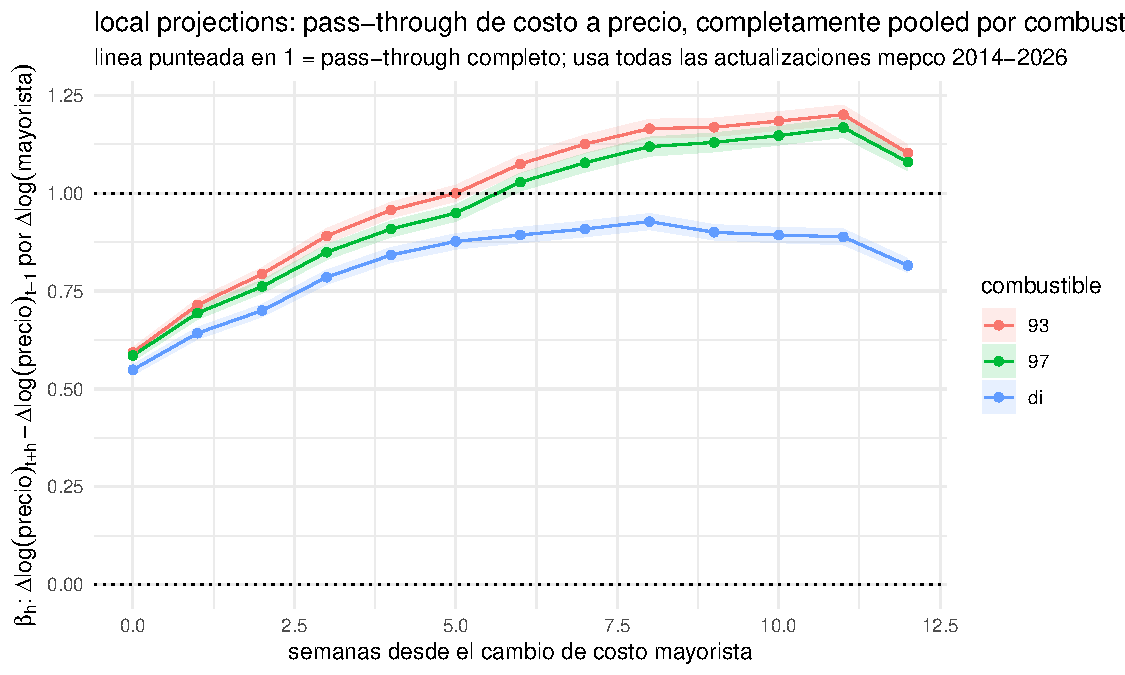
\includegraphics[width=0.85\textwidth]{../results/figures/lp_irf_fuel.pdf}
\caption{Funciones de impulso-respuesta por combustible,
ecuación~\eqref{eq:lp}. Bandas de confianza al 95\% con errores estándar
agrupados por estación.}
\label{fig:lp_fuel}
\end{figure}

\begin{figure}[htbp]
\centering
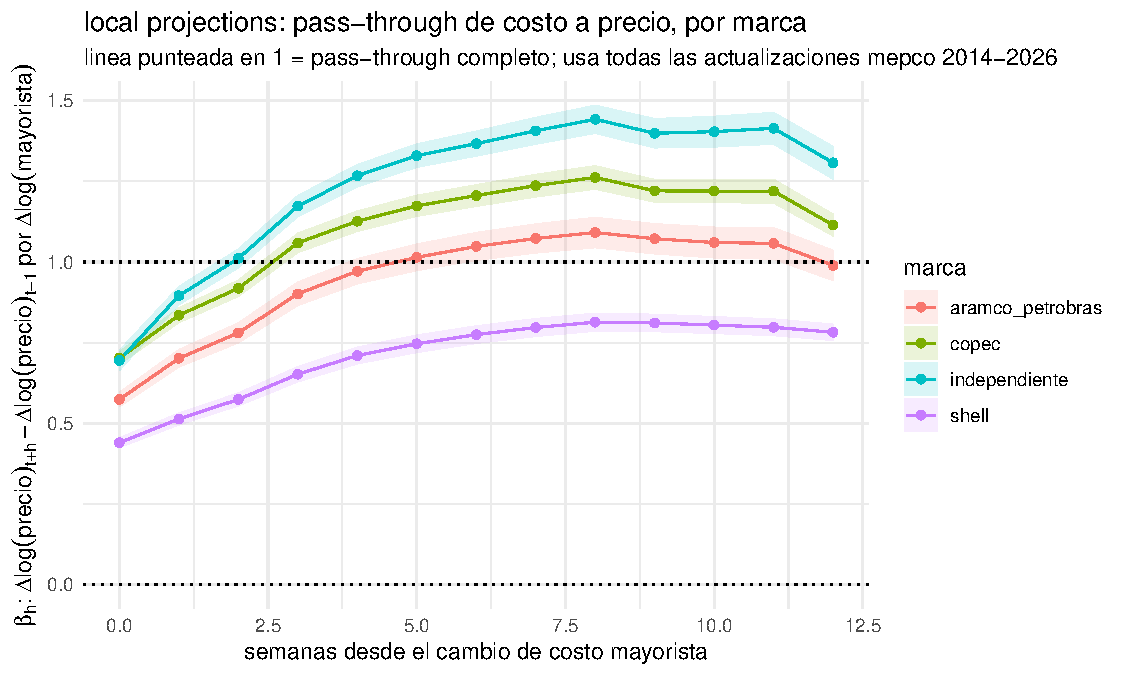
\includegraphics[width=0.85\textwidth]{../results/figures/lp_irf_brand.pdf}
\caption{Funciones de impulso-respuesta por marca (distribuidor modal).}
\label{fig:lp_brand}
\end{figure}

\begin{figure}[htbp]
\centering
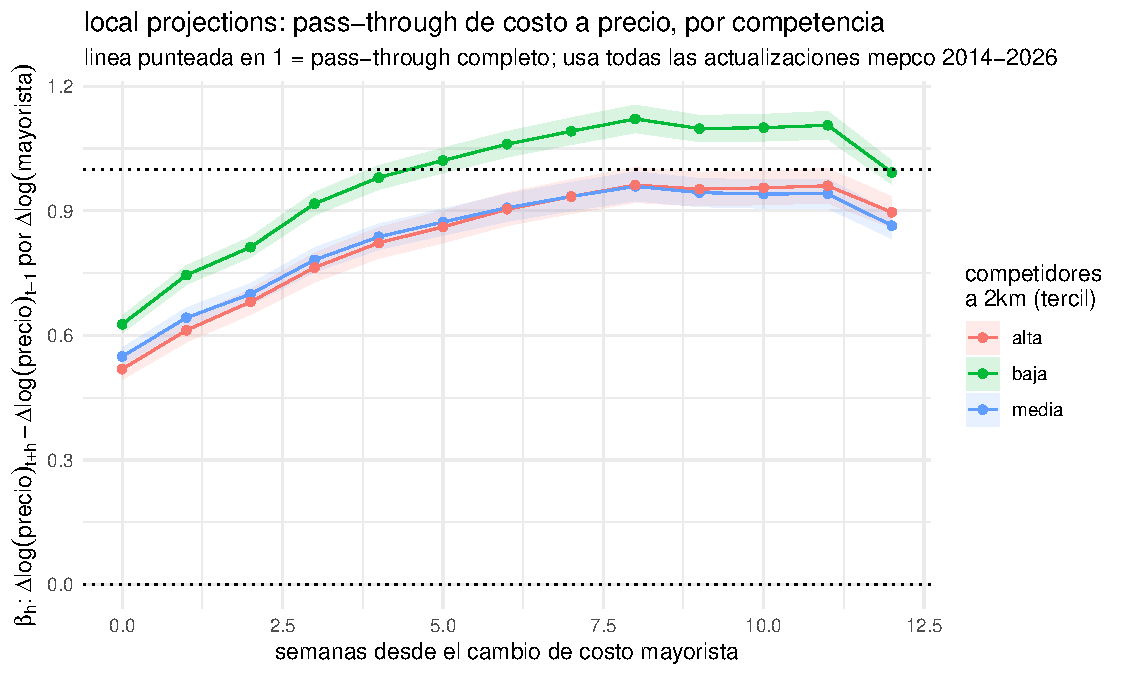
\includegraphics[width=0.85\textwidth]{../results/figures/lp_irf_competitors.pdf}
\caption{Funciones de impulso-respuesta por tercil de competidores dentro de
2 km.}
\label{fig:lp_comp}
\end{figure}

\begin{figure}[htbp]
\centering
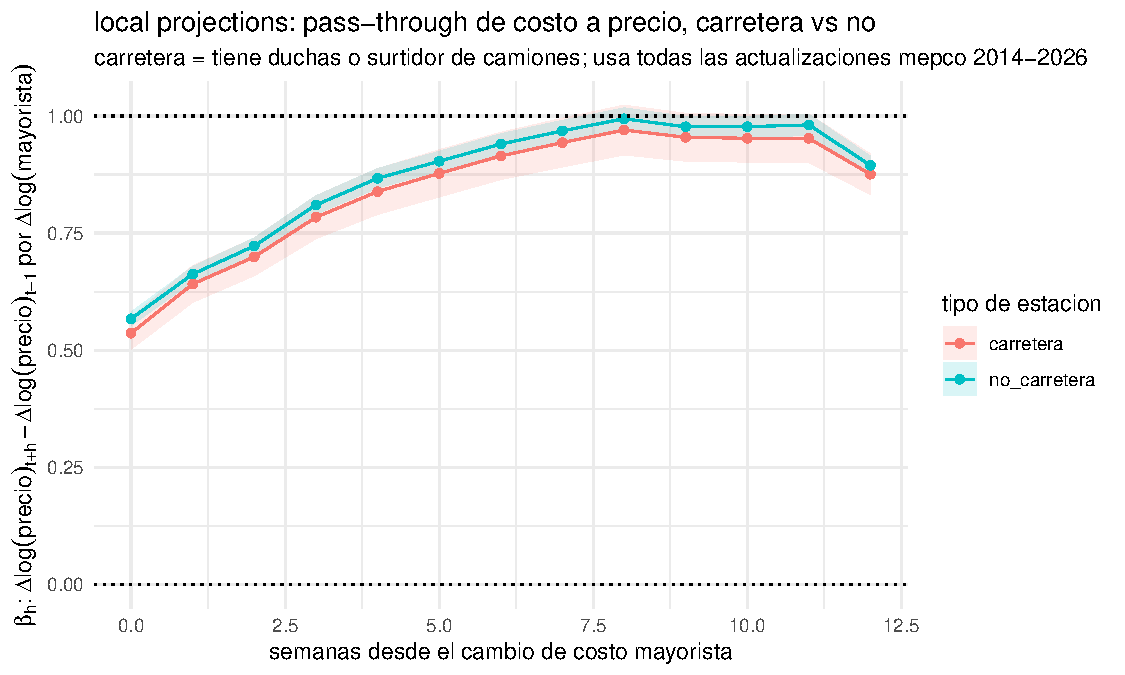
\includegraphics[width=0.85\textwidth]{../results/figures/lp_irf_carretera.pdf}\\[6pt]
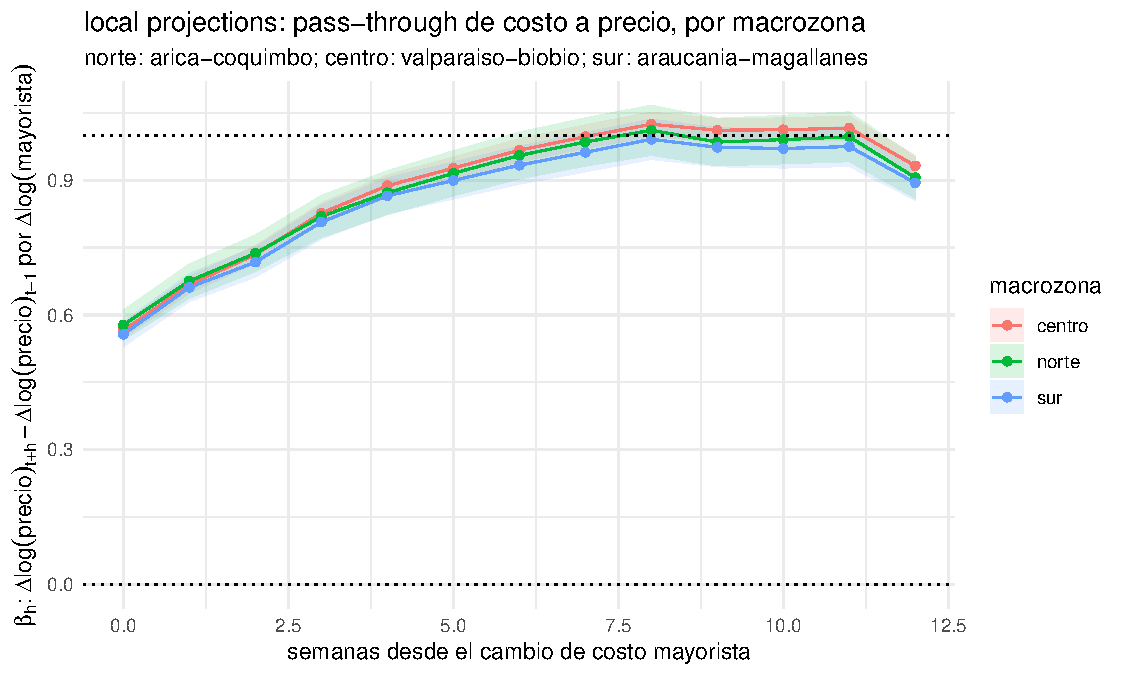
\includegraphics[width=0.85\textwidth]{../results/figures/lp_irf_macrozona.pdf}
\caption{Funciones de impulso-respuesta por tipo de estación (arriba) y por
macrozona (abajo).}
\label{fig:lp_carretera_macro}
\end{figure}

\section{Proyecciones locales del shock del MEPCO de marzo de 2026}
\label{sec:lp_evento}

El 26 de marzo de 2026 el MEPCO aplicó el mayor ajuste de su historia, con
alzas simultáneas en los tres combustibles cubiertos pero de tamaño muy
distinto (Tabla~\ref{tab:dosis}). Esta sección estima la respuesta minorista
a ese único evento usando el tamaño del alza de cada combustible como dosis.
Comparar respuestas de precios en niveles entre combustibles confundiría
responder más con haber recibido un shock más grande, y escalar por la dosis
corrige esa confusión.

\begin{table}[htbp]
\centering
\caption{Dosis del shock del 26 de marzo de 2026 por combustible.}
\label{tab:dosis}
\begin{tabular}{lccc}
\toprule
Combustible & Mayorista al 19/03 & Mayorista al 26/03 & $\Delta \log w_f$ \\
 & (\$/L) & (\$/L) & \\
\midrule
Gasolina 93 & 1.083,3 & 1.455,5 & 0,296 \\
Gasolina 97 & 1.133,1 & 1.524,6 & 0,297 \\
Diésel      & 831,2   & 1.411,5 & 0,530 \\
\bottomrule
\end{tabular}

\medskip
\begin{minipage}{0.8\textwidth}
\footnotesize
Nota: precios mayoristas con MEPCO. La dosis del diésel casi duplica la de
las gasolinas.
\end{minipage}
\end{table}

\subsection{Especificación}
\label{sec:lp_evento_especificacion}

La muestra se restringe a los pares estación-combustible activos durante
toda la ventana, con primera observación en o antes del 19 de marzo de 2026
y última al menos 12 semanas después del evento, para evitar efectos de
composición por entrada y salida. Quedan 4.938 pares.\footnote{El precio de
cada par se muestrea con la última observación disponible en la fecha previa
al shock y en cada fecha $26/03/2026 + 7h$ con $h = 0, \dots, 12$. Cuando
una estación reporta más de una vez el mismo día se conserva el último
reporte. Los grupos de heterogeneidad se fijan en la última observación
previa al shock de cada par.} Para cada horizonte se estima la regresión de
corte transversal

\begin{equation}
\label{eq:lp_evento}
\log p_{if,h} - \log p_{if,\mathrm{pre}}
= \alpha^{(h)} + \beta_h \, \Delta \log w_f + \varepsilon_{if}^{(h)},
\end{equation}

con errores estándar agrupados por estación. Con una sola fecha de shock no
hay variación temporal que explotar. La identificación de $\beta_h$ proviene
solo de los tres niveles de dosis entre combustibles y no es posible incluir
efectos fijos de estación ni controles por la historia del shock. El
intercepto absorbe el ajuste común a los tres combustibles, de modo que
$\beta_h$ es una pendiente dosis-respuesta entre combustibles y no el
traspaso estructural de la Sección~\ref{sec:lp}. Cualquier movimiento
mayorista posterior específico a un combustible carga directamente sobre
$\beta_h$, lo que resulta central para leer los horizontes largos.

\subsection{Resultados}
\label{sec:lp_evento_resultados}

La Tabla~\ref{tab:lp_evento_pooled} reporta la trayectoria agregada completa
y la Tabla~\ref{tab:lp_evento_het} los cortes por marca y competencia. Las
Figuras~\ref{fig:lp_evento_brand} y~\ref{fig:lp_evento_comp} muestran las
trayectorias con sus bandas de confianza.

\begin{table}[htbp]
\centering
\caption{Proyecciones locales del shock de marzo de 2026: trayectoria
agregada.}
\label{tab:lp_evento_pooled}
\begin{tabular}{ccc}
\toprule
Horizonte $h$ (semanas) & $\beta_h$ & EE \\
\midrule
0  & 0,811 & (0,007) \\
1  & 0,830 & (0,006) \\
2  & 0,838 & (0,005) \\
3  & 0,881 & (0,005) \\
4  & 0,889 & (0,004) \\
5  & 0,890 & (0,004) \\
6  & 0,777 & (0,004) \\
7  & 0,770 & (0,004) \\
8  & 0,769 & (0,004) \\
9  & 0,600 & (0,004) \\
10 & 0,589 & (0,004) \\
11 & 0,587 & (0,004) \\
12 & 0,494 & (0,005) \\
\bottomrule
\end{tabular}

\medskip
\begin{minipage}{0.8\textwidth}
\footnotesize
Nota: $\beta_h$ de la ecuación~\eqref{eq:lp_evento}, con 4.938 pares
estación-combustible en todos los horizontes. Errores estándar agrupados por
estación.
\end{minipage}
\end{table}

\begin{table}[htbp]
\centering
\caption{Proyecciones locales del shock de marzo de 2026: heterogeneidad.}
\label{tab:lp_evento_het}
\begin{tabular}{lcccccc}
\toprule
 & & \multicolumn{5}{c}{Horizonte $h$ (semanas)} \\
\cmidrule(lr){3-7}
 & $N$ & 0 & 2 & 4 & 8 & 12 \\
\midrule
\multicolumn{7}{l}{\emph{Panel A: marca (fijada antes del shock)}} \\
Copec             & 2.064 & 0,827 & 0,834 & 0,880 & 0,756 & 0,482 \\
                  &       & (0,007) & (0,004) & (0,004) & (0,004) & (0,004) \\
Shell             & 1.362 & 0,853 & 0,844 & 0,887 & 0,759 & 0,495 \\
                  &       & (0,007) & (0,006) & (0,006) & (0,006) & (0,008) \\
Aramco-Petrobras  & 896   & 0,782 & 0,799 & 0,857 & 0,740 & 0,452 \\
                  &       & (0,014) & (0,012) & (0,009) & (0,007) & (0,021) \\
Independientes    & 616   & 0,797 & 0,922 & 0,983 & 0,885 & 0,588 \\
                  &       & (0,033) & (0,025) & (0,024) & (0,021) & (0,019) \\
\addlinespace
\multicolumn{7}{l}{\emph{Panel B: competidores a 2 km (terciles)}} \\
Baja              & 1.863 & 0,789 & 0,823 & 0,876 & 0,759 & 0,488 \\
                  &       & (0,012) & (0,009) & (0,008) & (0,007) & (0,007) \\
Media             & 1.724 & 0,813 & 0,843 & 0,886 & 0,767 & 0,482 \\
                  &       & (0,013) & (0,006) & (0,006) & (0,006) & (0,011) \\
Alta              & 1.351 & 0,840 & 0,856 & 0,910 & 0,786 & 0,517 \\
                  &       & (0,011) & (0,009) & (0,007) & (0,007) & (0,009) \\
\bottomrule
\end{tabular}

\medskip
\begin{minipage}{0.92\textwidth}
\footnotesize
Nota: ecuación~\eqref{eq:lp_evento} estimada dentro de cada grupo. $N$ es el
número de pares estación-combustible. Errores estándar agrupados por
estación entre paréntesis.
\end{minipage}
\end{table}

La respuesta al evento es mucho más rápida que la respuesta promedio
histórica. El traspaso de impacto es 0,811 contra 0,565 de la
Sección~\ref{sec:lp} y alcanza un máximo de 0,890 en la quinta semana. Un
shock de esta magnitud y visibilidad pública se procesa más rápido que la
actualización semanal típica del MEPCO.

Desde la sexta semana el coeficiente cae en escalones (0,89 a 0,77, a 0,60 y
a 0,49). Esa caída no es una reversión del traspaso del shock de marzo sino
el reflejo de las actualizaciones posteriores del MEPCO, que la
ecuación~\eqref{eq:lp_evento} no puede controlar. El mayorista del diésel
bajó 46,9 \$/L el 7 de mayo, 65,0 \$/L el 28 de mayo y 117,5 \$/L el 18 de
junio, mientras las gasolinas quedaron casi planas hasta una baja de unos 95
\$/L el 18 de junio. Como las bajas posteriores se concentraron en el
combustible con la mayor dosis, la pendiente dosis-respuesta se aplana
mecánicamente y los escalones de la Tabla~\ref{tab:lp_evento_pooled}
coinciden una a una con esas fechas. La Figura~\ref{fig:lp_evento_brand}
confirma esta lectura, pues los escalones son comunes a las cuatro marcas y
ocurren en las mismas fechas, lo que descarta una reversión diferencial de
alguna red.

En heterogeneidad, las diferencias de impacto entre marcas son pequeñas
(entre 0,78 y 0,85) y contrastan con las brechas amplias del ejercicio
histórico. Shell no se rezaga frente a este shock (0,853 en el impacto, el
valor más alto entre marcas) y las independientes vuelven a mostrar el
traspaso más alto desde la segunda semana (0,983 en $h = 4$ contra 0,889 del
agregado). El gradiente de competencia se invierte respecto del ejercicio
histórico, con el tercil alto levemente por encima (0,840 contra 0,789 en el
impacto), aunque en la Figura~\ref{fig:lp_evento_comp} las tres trayectorias
se mueven en paralelo y la brecha entre terciles es un orden de magnitud
menor que los movimientos comunes. La lectura económica es que, ante un
shock grande y de conocimiento público, la velocidad de ajuste converge
entre tipos de estación y el entorno competitivo pierde el rol que juega
frente a las actualizaciones semanales pequeñas.

\begin{figure}[htbp]
\centering
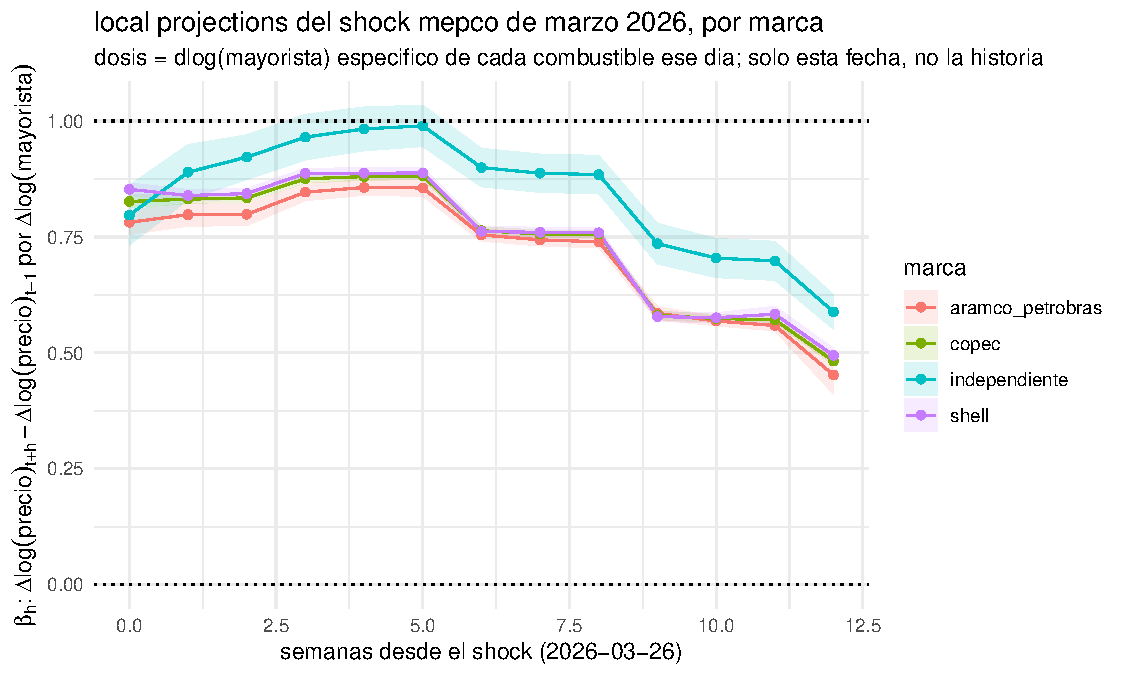
\includegraphics[width=0.85\textwidth]{../results/figures/lp_evento2026_brand.pdf}
\caption{Shock de marzo de 2026: respuesta por marca,
ecuación~\eqref{eq:lp_evento}.}
\label{fig:lp_evento_brand}
\end{figure}

\begin{figure}[htbp]
\centering
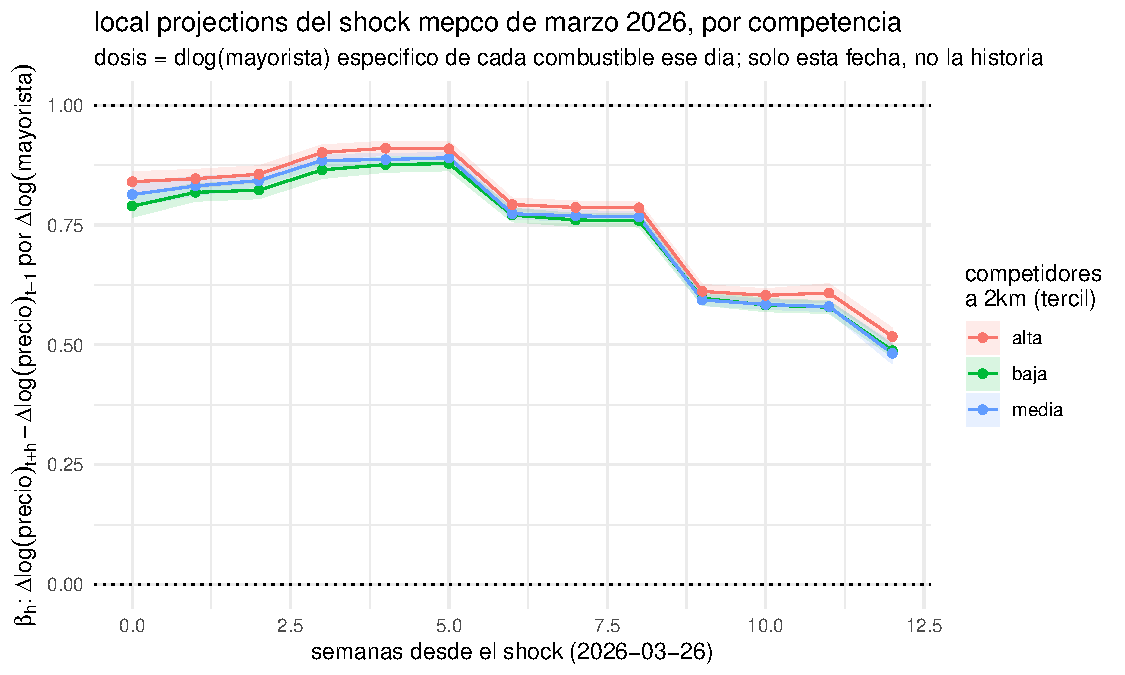
\includegraphics[width=0.85\textwidth]{../results/figures/lp_evento2026_competitors.pdf}
\caption{Shock de marzo de 2026: respuesta por tercil de competidores dentro
de 2 km.}
\label{fig:lp_evento_comp}
\end{figure}

\section{Interpretación conjunta: proyecciones locales y rezagos distribuidos}
\label{sec:conjunta}

Las proyecciones locales de la Sección~\ref{sec:lp} tienen una contraparte
natural de rezagos distribuidos, una sola regresión del cambio semanal del
precio sobre el shock contemporáneo y sus rezagos. Ambos estimadores usan la
misma grilla, los mismos efectos fijos y las mismas submuestras, de modo que
cualquier diferencia entre ellos es atribuible a la especificación y no a
los datos. Esta sección presenta el estimador de rezagos distribuidos,
documenta que difiere de las proyecciones locales en horizontes intermedios
y largos, y muestra que la diferencia no es una contradicción sino que cada
método estima un objeto económico distinto.

\subsection{Especificación}
\label{sec:dl_especificacion}

Se estima, para cada submuestra, la regresión única

\begin{equation}
\label{eq:dl}
\Delta \log p_{i,f,t}
= \alpha_{if}
+ \sum_{k=0}^{K} \theta_k \, \Delta \log w_{f,t-k}
+ \varepsilon_{i,f,t},
\qquad K = 26,
\end{equation}

con efectos fijos estación por combustible y errores estándar agrupados por
estación. La variable dependiente es el cambio semanal del precio, no la
diferencia acumulada de la ecuación~\eqref{eq:lp}, porque cada $\theta_k$ ya
lleva su propio horizonte. El traspaso acumulado a $h$ semanas es
$PT(h) = \sum_{k=0}^{h} \theta_k$ y su error estándar se calcula con la
matriz de varianzas y covarianzas completa del modelo, pues los $\theta_k$
están correlacionados entre sí.\footnote{Como robustez se estimó una
variante ARDL con rezagos de la propia variable dependiente. El traspaso de
largo plazo implícito, $\sum \theta_k / (1 - \sum \gamma_j) \approx
0{,}76$, es casi idéntico al de la especificación~\eqref{eq:dl}, al costo de
una colinealidad severa, por lo que se reporta la versión simple.}

\subsection{Resultados}
\label{sec:dl_resultados}

La Tabla~\ref{tab:lp_dl} compara el traspaso acumulado de ambos métodos en
el agregado y la Tabla~\ref{tab:lp_dl_het} lo hace por combustible, marca y
competencia. Las Figuras~\ref{fig:dl_fuel} y~\ref{fig:dl_het} muestran las
trayectorias del estimador de rezagos distribuidos.

\begin{table}[htbp]
\centering
\caption{Traspaso acumulado agregado: proyecciones locales contra rezagos
distribuidos.}
\label{tab:lp_dl}
\begin{tabular}{ccc}
\toprule
Horizonte $h$ (semanas) & LP: $\beta_h$ & DL: $PT(h)$ \\
\midrule
0  & 0,565 & 0,560 \\
   & (0,007) & (0,007) \\
2  & 0,732 & 0,638 \\
   & (0,008) & (0,006) \\
4  & 0,882 & 0,658 \\
   & (0,010) & (0,006) \\
8  & 1,017 & 0,671 \\
   & (0,011) & (0,005) \\
12 & 0,922 & 0,654 \\
   & (0,009) & (0,006) \\
26 &       & 0,678 \\
   &       & (0,005) \\
\bottomrule
\end{tabular}

\medskip
\begin{minipage}{0.8\textwidth}
\footnotesize
Nota: LP corresponde a $\beta_h$ de la ecuación~\eqref{eq:lp} y DL a
$PT(h) = \sum_{k \le h} \theta_k$ de la ecuación~\eqref{eq:dl}, ambas sobre
la misma grilla y con errores estándar agrupados por estación entre
paréntesis. El horizonte máximo de las proyecciones locales es 12 semanas.
\end{minipage}
\end{table}

\begin{table}[htbp]
\centering
\caption{Traspaso de largo plazo por grupo: proyecciones locales contra
rezagos distribuidos.}
\label{tab:lp_dl_het}
\begin{tabular}{lccc}
\toprule
 & LP: $\beta_8$ & LP: $\beta_{12}$ & DL: $PT(26)$ \\
\midrule
\multicolumn{4}{l}{\emph{Panel A: combustible}} \\
Gasolina 93       & 1,165 (0,012) & 1,103 (0,011) & 0,691 (0,006) \\
Gasolina 97       & 1,119 (0,012) & 1,080 (0,011) & 0,663 (0,006) \\
Diésel            & 0,928 (0,011) & 0,815 (0,009) & 0,685 (0,005) \\
\addlinespace
\multicolumn{4}{l}{\emph{Panel B: marca}} \\
Copec             & 1,199 (0,018) & 1,043 (0,016) & 0,767 (0,007) \\
Shell             & 0,759 (0,013) & 0,733 (0,012) & 0,525 (0,006) \\
Aramco-Petrobras  & 1,019 (0,022) & 0,927 (0,021) & 0,699 (0,009) \\
Independientes    & 1,353 (0,018) & 1,172 (0,020) & 0,846 (0,009) \\
\addlinespace
\multicolumn{4}{l}{\emph{Panel C: competidores a 2 km}} \\
Baja              & 1,121 (0,017) & 0,992 (0,014) & 0,730 (0,008) \\
Media             & 0,959 (0,018) & 0,864 (0,016) & 0,662 (0,009) \\
Alta              & 0,962 (0,021) & 0,896 (0,019) & 0,639 (0,010) \\
\bottomrule
\end{tabular}

\medskip
\begin{minipage}{0.92\textwidth}
\footnotesize
Nota: errores estándar agrupados por estación entre paréntesis. En carretera
y macrozona el patrón replica el de las proyecciones locales, con $PT(26)$
de 0,661 en carretera contra 0,675 en el resto y de 0,652, 0,687 y 0,664 en
norte, centro y sur.
\end{minipage}
\end{table}

Los dos estimadores coinciden donde deben coincidir, en el impacto (0,565 y
0,560), y divergen de forma creciente con el horizonte, hasta 1,017 contra
0,671 en la octava semana, una razón de 1,52. La forma también difiere. En
la Figura~\ref{fig:dl_fuel} el traspaso acumulado converge en unas cuatro
semanas y queda plano, sin la joroba ni la reversión de las proyecciones
locales, con los tres combustibles superpuestos. En la
Figura~\ref{fig:dl_het} el ordenamiento por marca y competencia queda
establecido desde las primeras semanas y las bandas de Shell y de las
independientes no se traslapan con el resto en ningún horizonte.

\subsection{Por qué difieren y qué estima cada método}
\label{sec:dl_interpretacion}

La diferencia está en qué mantiene fijo cada método. El estimador de rezagos
distribuidos condiciona en toda la trayectoria del mayorista, de modo que
$PT(h)$ es la respuesta acumulada a un alza unitaria aislada. Las
proyecciones locales controlan por los rezagos del shock, lo que purga la
parte predecible desde el pasado, pero nada pueden hacer con las alzas
futuras que la innovación de hoy anticipa. Como el MEPCO se mueve en rachas,
$\beta_h$ acumula también el traspaso de las alzas posteriores
correlacionadas. Las proyecciones locales estiman la respuesta a una
innovación del proceso mayorista, trayectoria completa incluida, y los
rezagos distribuidos la respuesta a un peso de costo que llega solo.

Los datos respaldan esta lectura cuantitativamente. Un AR(13) ajustado a
$\Delta \log w_{f,t}$ implica que una innovación unitaria deja el nivel
mayorista entre 1,6 y 1,8 unidades sobre su nivel inicial ocho semanas
después, magnitud comparable con la razón de 1,52 entre ambos estimadores en
esa semana. Además, esa razón es casi constante entre grupos, entre 1,45 y
1,60 para todas las marcas y terciles de la Tabla~\ref{tab:lp_dl_het}. Si la
brecha reflejara conducta de algún grupo debería variar entre ellos. Un
factor común del proceso de shocks, idéntico para todos, la explica de
manera parsimoniosa.

Tres conclusiones económicas se desprenden. Primero, el aparente
sobre-traspaso de las proyecciones locales no es evidencia de demanda
convexa ni de sobrerreacción de márgenes. Desaparece al aislar el shock y
$PT(h)$ no supera 1 en ningún grupo ni horizonte. Segundo, la brecha entre
combustibles de las proyecciones locales es una propiedad del proceso de
shocks y no de la conducta minorista. El momentum del mayorista del diésel
es menor que el de las gasolinas (multiplicador de 1,59 contra 1,78 a la
octava semana) y, una vez descontado, el traspaso de largo plazo es casi
idéntico entre combustibles (0,691, 0,663 y 0,685). Tercero, la
heterogeneidad por marca y competencia sobrevive intacta al cambio de
método, con el mismo ordenamiento. Shell traspasa 0,525 de un peso aislado
contra 0,846 de las independientes, y el tercil de baja competencia 0,730
contra 0,639 del de alta. Esa estabilidad permite atribuir las brechas a
conducta de fijación de precios y no a diferencias en los shocks que cada
grupo enfrenta.

En síntesis, cada método responde una pregunta distinta. Los rezagos
distribuidos responden cuánto de un peso de costo aislado llega al surtidor,
alrededor de 0,68 incluso a seis meses, un traspaso incompleto. Las
proyecciones locales responden qué le ocurre al precio tras una alza típica
del MEPCO, dado que las alzas vienen en rachas, aproximadamente uno a uno al
cabo de dos meses. Para inferencia sobre poder de mercado e incidencia el
objeto relevante es el primero. Para pronóstico y comunicación de política,
el segundo.\footnote{La equivalencia asintótica entre proyecciones locales y
representaciones autorregresivas (Plagborg-Møller y Wolf, 2021) requiere
estructuras de rezagos irrestrictas. Aquí ambas están deliberadamente
restringidas y la diferencia entre ellas es informativa sobre la
persistencia del proceso de costos, no un fallo de especificación.}

\begin{figure}[htbp]
\centering
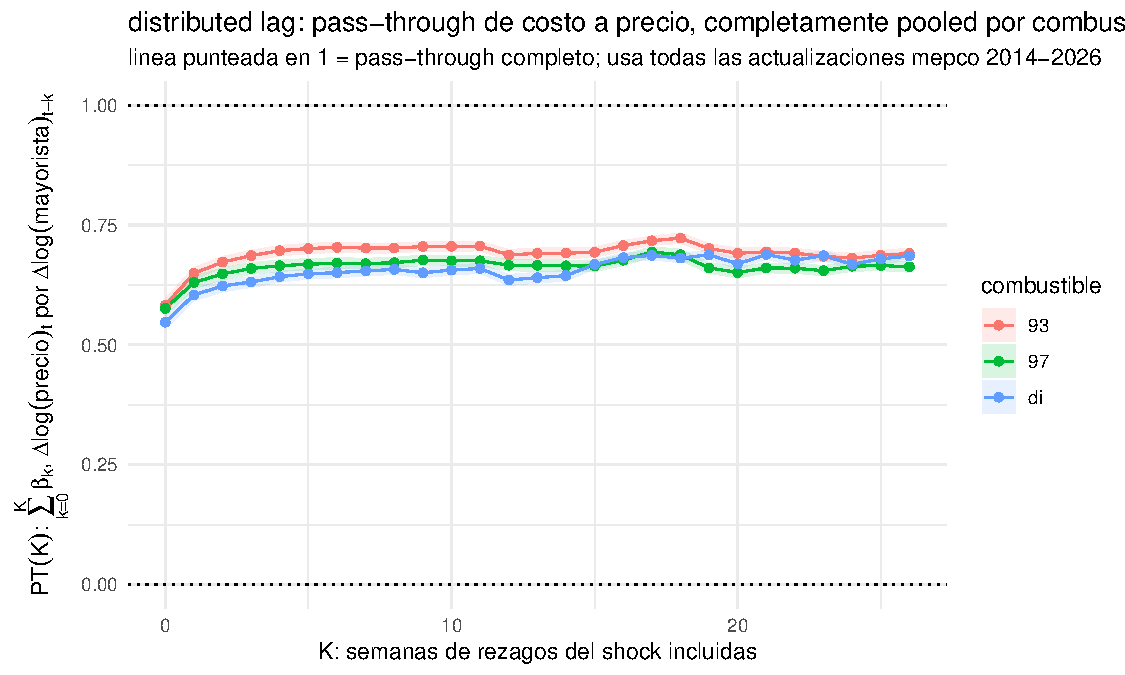
\includegraphics[width=0.85\textwidth]{../results/figures/dl_irf_fuel.pdf}
\caption{Rezagos distribuidos: traspaso acumulado $PT(K)$ por combustible,
ecuación~\eqref{eq:dl}. Bandas de confianza al 95\% con errores estándar
agrupados por estación.}
\label{fig:dl_fuel}
\end{figure}

\begin{figure}[htbp]
\centering
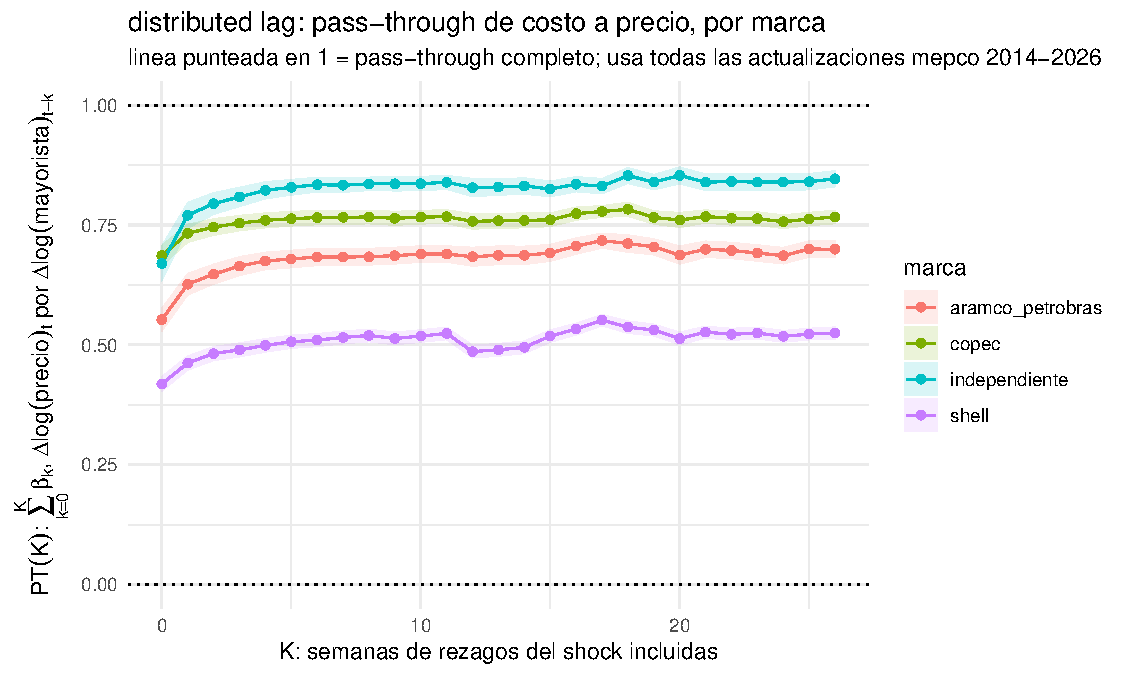
\includegraphics[width=0.85\textwidth]{../results/figures/dl_irf_brand.pdf}\\[6pt]
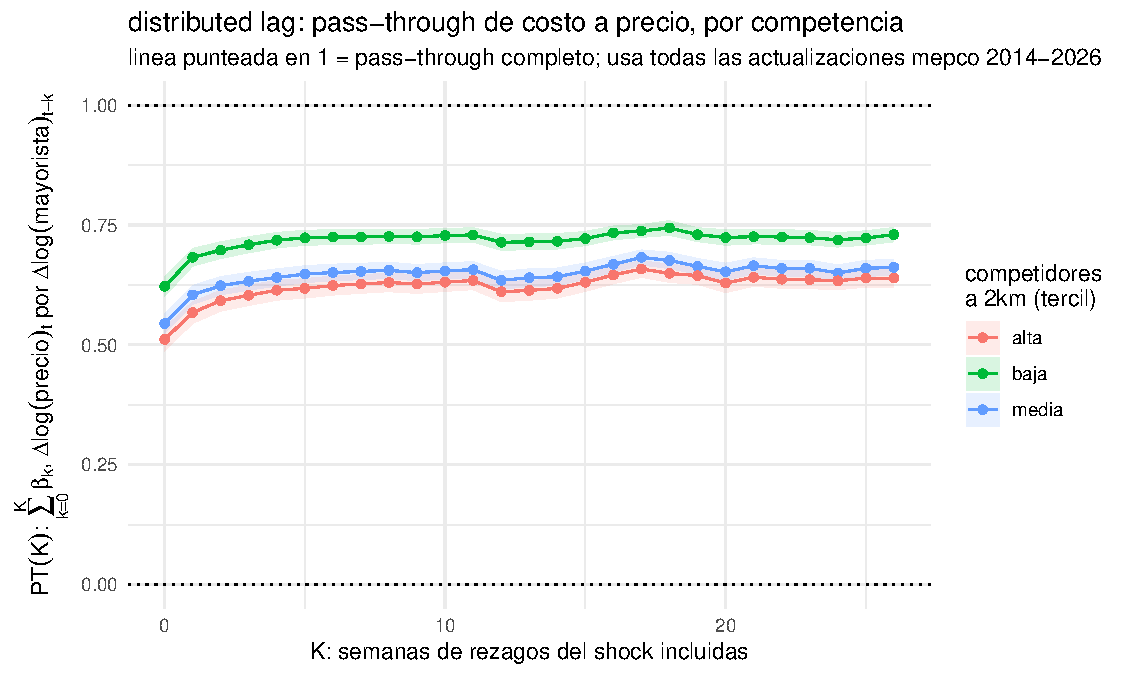
\includegraphics[width=0.85\textwidth]{../results/figures/dl_irf_competitors.pdf}
\caption{Rezagos distribuidos: traspaso acumulado por marca (arriba) y por
tercil de competidores dentro de 2 km (abajo).}
\label{fig:dl_het}
\end{figure}

\section{Márgenes minoristas en torno al shock de marzo de 2026}
\label{sec:margenes}

Esta sección complementa las elasticidades con un análisis descriptivo en
niveles. Se estudia el margen minorista, definido como el precio de venta
menos el costo mayorista con MEPCO vigente, en pesos por litro, en una
ventana de 14 semanas a cada lado del shock de marzo de 2026. El margen así
definido es una brecha bruta respecto de la referencia mayorista pública y
no un margen contable, de modo que la información está en sus comparaciones
entre grupos y en el tiempo, no en su nivel absoluto.

\subsection{Construcción}
\label{sec:margenes_construccion}

La muestra se restringe a las estaciones activas durante toda la ventana
(1.564 reportan en la semana del shock). La agregación usa medianas en dos
pasos, primero dentro de cada estación y semana y luego entre estaciones de
cada grupo, de modo que una estación que reporta con más frecuencia no pese
más. Las bandas de las figuras son el rango intercuartílico entre estaciones
y miden dispersión transversal, no un intervalo de confianza. La marca y el
tercil de competidores se fijan antes del shock. La elección de medianas
responde a un problema de outliers detectado en la
construcción.\footnote{Unas 665 observaciones presentan márgenes sobre
\$400/L, muy por encima del rango típico de \$100 a \$180/L, todas con
precios recién reportados. La revisión identificó dos orígenes. Uno es un
efecto regional real, pues Aysén y Magallanes operan con márgenes de \$150 a
\$180/L en toda su muestra contra \$80 a \$95/L en el centro del país,
consistente con costos de transporte. El otro son errores aislados de
reporte, como ocho estaciones de Quilpué y Villa Alemana que reportaron el
25 de marzo de 2026 un diésel idéntico de \$1.530/L, un día antes de que el
mayorista subiera, un aparente error de carga masiva. Solo cerca del 21\% de
esas observaciones tiene la firma inequívoca de un error, por lo que se
optó por medianas en vez de una regla global de depuración. El único rastro
visible es la banda superior del diésel en la semana previa al shock, cuya
mediana no se ve afectada.}

\subsection{Resultados}
\label{sec:margenes_resultados}

La Tabla~\ref{tab:margenes} resume la trayectoria del margen mediano por
marca, combustible y competencia. Las Figuras~\ref{fig:tijera}
a~\ref{fig:margen_comp} muestran la evolución semanal.

\begin{table}[htbp]
\centering
\caption{Margen minorista mediano en torno al shock de marzo de 2026
(\$/L).}
\label{tab:margenes}
\begin{tabular}{lcccccc}
\toprule
 & $N$ & Base & Sem.\ 0 & Sem.\ 4 & Mínimo (sem.) & Sem.\ 14 \\
\midrule
\multicolumn{7}{l}{\emph{Panel A: marca}} \\
Copec             & 638   & 128,2 & 128,5 & 176,2 & 57,3 (11)  & 175,5 \\
Shell             & 447   & 127,9 & 125,5 & 171,6 & 69,4 (11)  & 171,5 \\
Aramco-Petrobras  & 275   & 132,8 & 135,5 & 172,3 & 124,3 (8)  & 174,8 \\
Independientes    & 204   & 115,8 & 117,8 & 113,2 & 89,0 (11)  & 147,6 \\
\addlinespace
\multicolumn{7}{l}{\emph{Panel B: combustible}} \\
Gasolina 93       & 1.537 & 120,5 & 123,5 & 173,3 & 69,0 (11)  & 175,5 \\
Gasolina 97       & 1.392 & 133,5 & 141,4 & 179,1 & 56,1 (11)  & 181,8 \\
Diésel            & 1.553 & 153,6 & 123,5 & 161,1 & 65,4 (11)  & 163,9 \\
\addlinespace
\multicolumn{7}{l}{\emph{Panel C: competidores a 2 km (terciles)}} \\
Baja              & 586   & 132,5 & 137,2 & 177,3 & 83,9 (11)  & 176,0 \\
Media             & 454   & 126,0 & 120,0 & 175,8 & 84,7 (11)  & 181,5 \\
Alta              & 524   & 119,5 & 111,5 & 166,2 & 74,8 (11)  & 170,8 \\
\bottomrule
\end{tabular}

\medskip
\begin{minipage}{0.95\textwidth}
\footnotesize
Nota: mediana entre estaciones de la mediana estación-semana del margen. $N$
es el número de estaciones (pares estación-combustible en el Panel B) que
reportan en la semana 0. Base es el promedio de las semanas $-4$ a $-1$.
Mínimo es el menor valor posterior al shock, con su semana entre paréntesis.
\end{minipage}
\end{table}

La ventana tiene cuatro fases. Primero, en la semana del shock el margen de
las gasolinas casi no se mueve (Copec pasa de 128,2 a 128,5), señal de que
el alza se traspasó al surtidor dentro de la misma semana. Es la contraparte
en niveles del traspaso de impacto de 0,81 de la
Sección~\ref{sec:lp_evento}. La excepción es el diésel, que se comprime
cerca de \$30/L en la semana 0 tras recibir una dosis casi doble, y ya en la
semana 1 estaba recuperado. Segundo, entre las semanas 1 y 5 los márgenes de
las tres grandes redes superan su base entre \$34 y \$48/L, un
sobre-traspaso transitorio en pesos coherente con las elasticidades sobre 1
de la Sección~\ref{sec:lp}. Tercero, entre las semanas 8 y 11 los márgenes
caen muy por debajo de la base en todos los grupos, con mínimo casi
universal en la semana 11, justo el tramo en que el mayorista del diésel
acumulaba bajas. Los precios minoristas cayeron más y más rápido que la
referencia vigente. Cuarto, tras la baja mayorista del 18 de junio (semana
12) los márgenes se reexpanden de inmediato y cierran la ventana entre \$32
y \$47/L sobre la base, porque ante una baja de costo el precio la sigue con
rezago y ese rezago es margen. La asimetría entre alzas y bajas se estima
formalmente en la Sección~\ref{sec:asimetrias}.

La Figura~\ref{fig:tijera} muestra la mecánica completa. El costo salta en
la semana 0, el precio lo alcanza en una o dos semanas, la brecha vertical
se estrecha entre las semanas 8 y 11 y se reabre tras la baja de la semana
12. La tijera del diésel es la de mayor amplitud en ambas direcciones,
consistente con su dosis mayor. En niveles
(Figura~\ref{fig:margen_marca}) las cuatro marcas parten de bases similares,
entre \$116 y \$133/L, así que las diferencias de conducta están en la
dinámica. La versión normalizada (Figura~\ref{fig:margen_norm}) muestra dos
contrastes. En la compresión de las semanas 8 a 11, Copec cae hasta \$71/L
bajo su base, Shell \$59/L y las independientes \$27/L, mientras
Aramco-Petrobras apenas se comprime (\$8,5/L), es decir, sostuvo sus precios
en el tramo de bajas en que el resto los recortaba. Y las independientes son
las únicas sin sobre-expansión en las semanas 1 a 5, porque movieron sus
precios junto con el costo, en línea con su traspaso alto y rápido de las
secciones anteriores.

Por combustible (Figura~\ref{fig:margen_fuel}), el diésel parte con el
margen base más alto (\$153,6/L contra \$120,5/L de la 93) y es el más
volátil de la ventana, como corresponde al combustible que recibió la mayor
alza y las mayores bajas. Por competencia
(Figura~\ref{fig:margen_comp}), el corte muestra un gradiente de nivel más
que de dinámica. El tercil de alta competencia opera con el margen más bajo
en casi toda la ventana (base de \$119,5/L contra \$132,5/L del tercil bajo)
y las tres trayectorias se mueven en paralelo. La lectura económica es la
esperable de un modelo de competencia espacial. La densidad de rivales
comprime el nivel del margen de manera persistente, pero la dinámica de
ajuste frente a un shock agregado y público es común a todos los entornos
competitivos.

\begin{figure}[htbp]
\centering
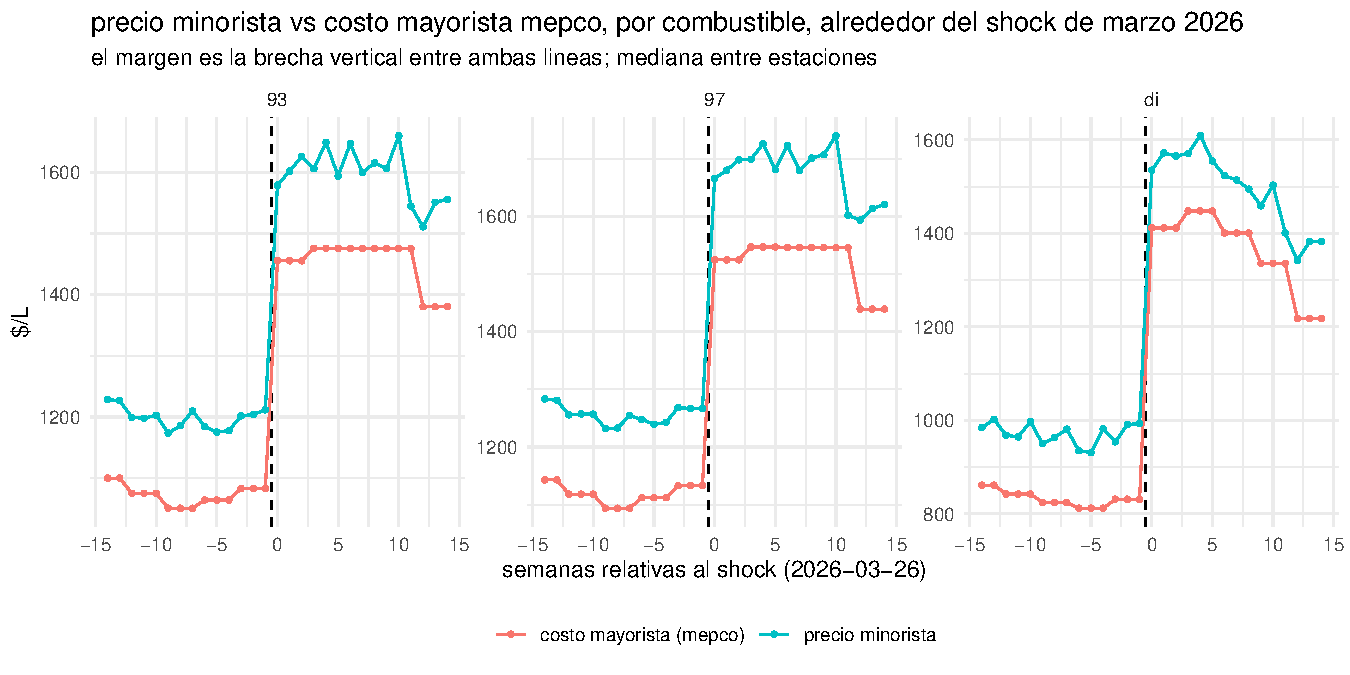
\includegraphics[width=\textwidth]{../results/figures/price_cost_by_fuel_week.pdf}
\caption{Precio minorista y costo mayorista MEPCO por combustible en torno
al shock de marzo de 2026. Medianas entre estaciones. El margen es la brecha
vertical entre ambas líneas.}
\label{fig:tijera}
\end{figure}

\begin{figure}[htbp]
\centering
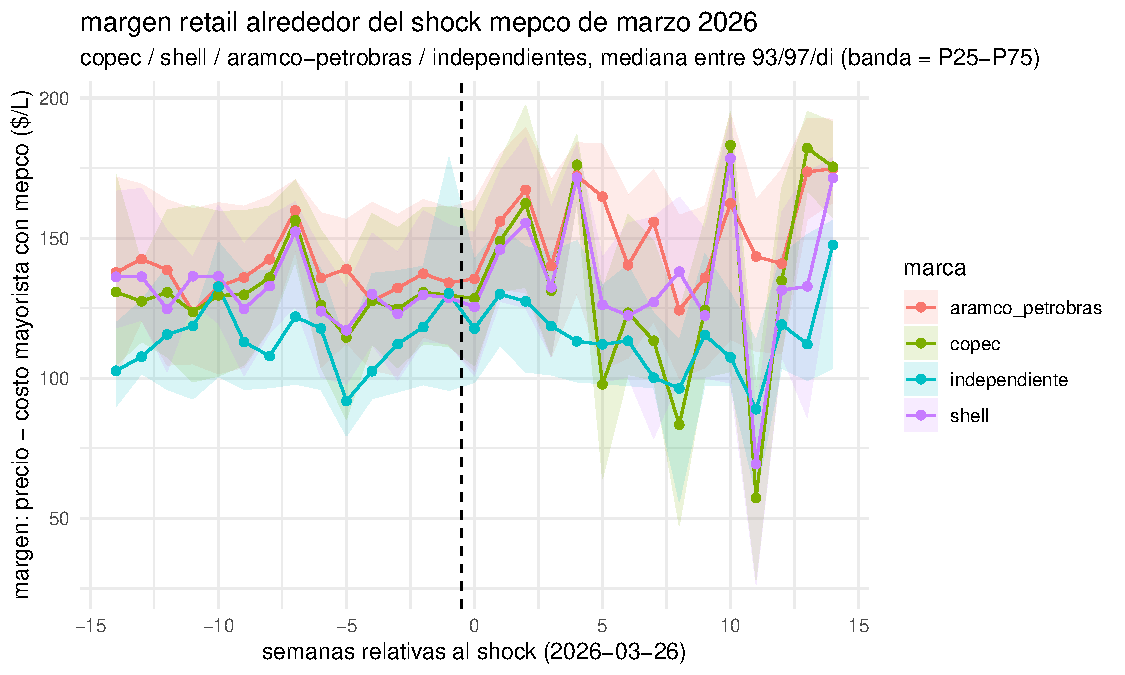
\includegraphics[width=0.85\textwidth]{../results/figures/margin_by_brand_week.pdf}
\caption{Margen minorista mediano por marca. Banda: rango intercuartílico
entre estaciones.}
\label{fig:margen_marca}
\end{figure}

\begin{figure}[htbp]
\centering
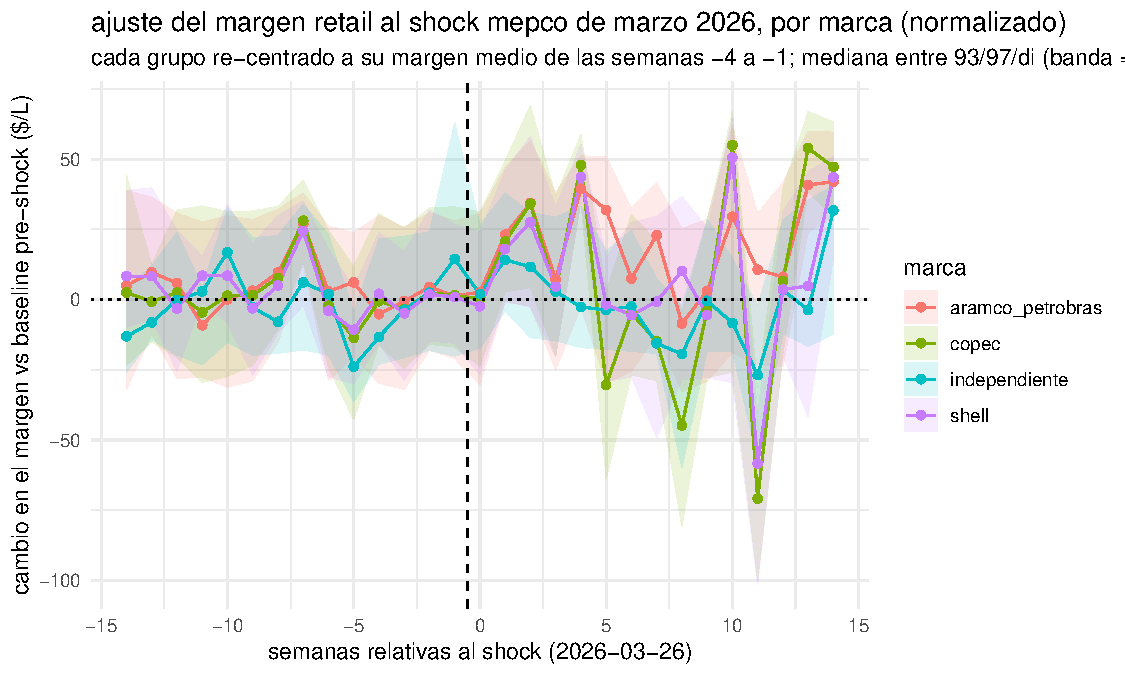
\includegraphics[width=0.85\textwidth]{../results/figures/margin_by_brand_week_normalized.pdf}
\caption{Cambio del margen respecto de la base propia de cada marca
(promedio de las semanas $-4$ a $-1$).}
\label{fig:margen_norm}
\end{figure}

\begin{figure}[htbp]
\centering
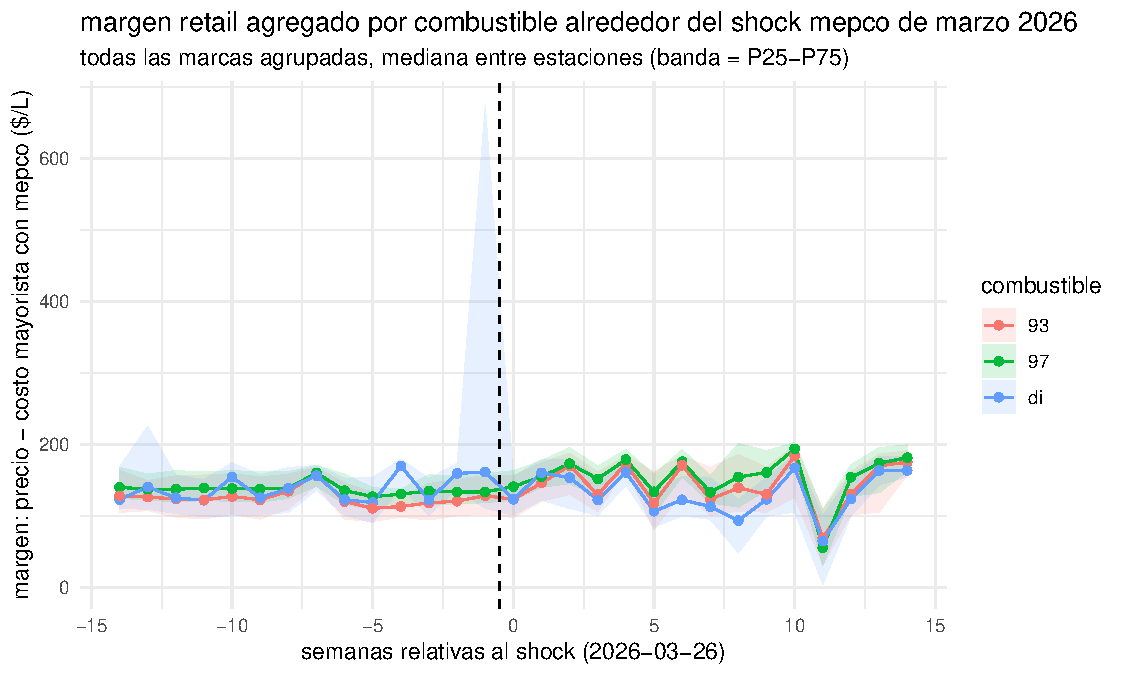
\includegraphics[width=0.85\textwidth]{../results/figures/margin_by_fuel_week.pdf}
\caption{Margen minorista mediano por combustible. Banda: rango
intercuartílico entre estaciones.}
\label{fig:margen_fuel}
\end{figure}

\begin{figure}[htbp]
\centering
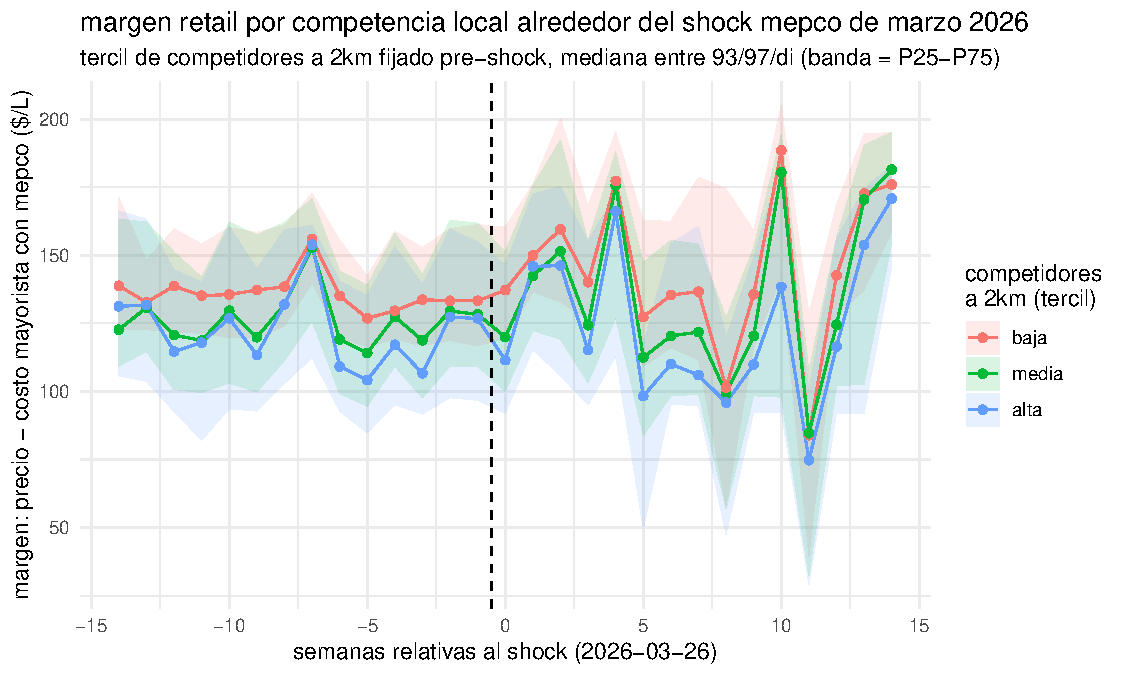
\includegraphics[width=0.85\textwidth]{../results/figures/margin_by_competition_week.pdf}
\caption{Margen minorista mediano por tercil de competidores dentro de 2 km
(fijado antes del shock). Banda: rango intercuartílico entre estaciones.}
\label{fig:margen_comp}
\end{figure}

\section{Asimetrías en el traspaso: \emph{rockets and feathers}}
\label{sec:asimetrias}

Esta sección estima si el traspaso es más rápido o más completo cuando el
costo sube que cuando baja, la pregunta central de la literatura de
\emph{rockets and feathers}. El hallazgo típico en
combustibles es que los precios suben como cohetes y bajan como plumas, un
patrón atribuido a costos de búsqueda o a colusión tácita. Se usan dos
diseños complementarios sobre la misma grilla semanal, y el segundo es la
especificación preferida.

\subsection{Especificaciones}
\label{sec:asimetrias_especificacion}

El primer diseño parte la muestra según el signo de $\Delta \log w_{f,t}$ en
la semana de origen y estima, para cada signo $s$ y horizonte $h$,

\begin{equation}
\label{eq:rf_split}
\log p_{i,f,t+h} - \log p_{i,f,t-1}
= \alpha_{if}^{(h,s)}
+ \beta_h^{(s)} \left( \log w_{f,t+h} - \log w_{f,t-1} \right)
+ \varepsilon_{i,f,t+h},
\qquad s \in \{\text{sube}, \text{baja}\},
\end{equation}

con efectos fijos estación por combustible y errores estándar agrupados por
estación. El regresor es el cambio mayorista acumulado sobre la misma
ventana que la variable dependiente, no el shock de la semana de origen,
para que $\beta_h^{(s)}$ sea la elasticidad al movimiento de costo
efectivamente realizado.\footnote{El shock de la semana de origen está
correlacionado entre 0,40 y 0,44 con los movimientos posteriores del
mayorista. Usarlo solo como regresor a horizontes largos lo convierte en
proxy de un movimiento acumulado mayor e infla $\beta_h$. Una versión
preliminar entregaba coeficientes sobre 2 para las bajas en $h = 8$, sin
sentido económico. El regresor acumulado es la solución estándar, análoga a
las regresiones de traspaso de tipo de cambio. Las semanas sin cambio del
mayorista se excluyen.}

El segundo diseño evita partir la muestra, porque condicionar en el signo de
origen selecciona trayectorias de costo distintas para cada submuestra y
puede fabricar asimetría espuria. Siguiendo a Borenstein, Cameron y Gilbert
(1997), cada paso semanal del mayorista se separa en su parte positiva y
negativa y ambas se acumulan por separado sobre la ventana:

\begin{equation}
\label{eq:rf_decomp}
\log p_{i,f,t+h} - \log p_{i,f,t-1}
= \alpha_{if}^{(h)}
+ \beta_h^{+} W^{+}_{f,t,h}
+ \beta_h^{-} W^{-}_{f,t,h}
+ \varepsilon_{i,f,t+h},
\end{equation}

donde $W^{\pm}_{f,t,h} = \sum_{k=0}^{h} \max/\min\{\Delta \log w_{f,t+k},
0\}$, con $W^{+} + W^{-}$ igual al regresor de la
ecuación~\eqref{eq:rf_split}. La regresión es una sola (3.238.217
observaciones) y la asimetría de interés es $\beta_h^{+} - \beta_h^{-}$,
positiva bajo el patrón clásico. Su error estándar usa la matriz de
varianzas y covarianzas conjunta agrupada por estación, de modo que el
contraste es una prueba formal sobre la diferencia. Ambos diseños se
reestiman por marca y por tercil de competidores a 2 km, etiquetados poca,
media y mucha competencia para no confundir con el sentido del shock.

\subsection{Resultados}
\label{sec:asimetrias_resultados}

La Tabla~\ref{tab:rf_split} presenta la partición por signo, la
Tabla~\ref{tab:rf_decomp} la descomposición agregada y la
Tabla~\ref{tab:rf_asym} la asimetría por subgrupo. Las
Figuras~\ref{fig:rf_irf} a~\ref{fig:rf_asym} muestran las trayectorias.

\begin{table}[htbp]
\centering
\caption{Traspaso según el signo del shock de la semana de origen (partición
muestral).}
\label{tab:rf_split}
\begin{tabular}{lcccccc}
\toprule
 & \multicolumn{6}{c}{Horizonte $h$ (semanas)} \\
\cmidrule(lr){2-7}
Origen & 0 & 1 & 2 & 4 & 8 & 12 \\
\midrule
Mayorista baja & 0,724 & 0,776 & 0,776 & 0,782 & 0,802 & 0,783 \\
               & (0,004) & (0,003) & (0,002) & (0,002) & (0,002) & (0,002) \\
Mayorista sube & 0,531 & 0,562 & 0,590 & 0,695 & 0,765 & 0,800 \\
               & (0,008) & (0,008) & (0,007) & (0,006) & (0,003) & (0,002) \\
\bottomrule
\end{tabular}

\medskip
\begin{minipage}{0.92\textwidth}
\footnotesize
Nota: $\beta_h^{(s)}$ de la ecuación~\eqref{eq:rf_split}, con errores
estándar agrupados por estación entre paréntesis. Submuestras de 1.134.657
(baja) y 1.459.510 (sube) observaciones.
\end{minipage}
\end{table}

\begin{table}[htbp]
\centering
\caption{Descomposición de alzas y bajas en una sola regresión (agregado).}
\label{tab:rf_decomp}
\begin{tabular}{cccccc}
\toprule
Horizonte $h$ & $\beta_h^{+}$ (alzas) & $\beta_h^{-}$ (bajas) &
$\beta_h^{+} - \beta_h^{-}$ & EE & $t$ \\
\midrule
0  & 0,542 & 0,779 & $-$0,237 & (0,008) & $-$30,1 \\
1  & 0,664 & 0,823 & $-$0,158 & (0,007) & $-$21,4 \\
2  & 0,717 & 0,832 & $-$0,115 & (0,007) & $-$16,2 \\
4  & 0,743 & 0,829 & $-$0,086 & (0,007) & $-$13,1 \\
8  & 0,786 & 0,825 & $-$0,038 & (0,005) & $-$7,3 \\
12 & 0,802 & 0,833 & $-$0,031 & (0,005) & $-$6,8 \\
\bottomrule
\end{tabular}

\medskip
\begin{minipage}{0.92\textwidth}
\footnotesize
Nota: ecuación~\eqref{eq:rf_decomp} sobre la muestra completa (3.238.217
observaciones), sin partición. Errores estándar de la diferencia calculados
con la matriz de varianzas y covarianzas conjunta, agrupada por estación.
Errores estándar de $\beta_h^{+}$ y $\beta_h^{-}$ entre 0,002 y 0,007.
\end{minipage}
\end{table}

\begin{table}[htbp]
\centering
\caption{Asimetría $\beta_h^{+} - \beta_h^{-}$ por subgrupo.}
\label{tab:rf_asym}
\begin{tabular}{lcccc}
\toprule
 & \multicolumn{4}{c}{Horizonte $h$ (semanas)} \\
\cmidrule(lr){2-5}
 & 0 & 4 & 8 & 12 \\
\midrule
\multicolumn{5}{l}{\emph{Panel A: competidores a 2 km (terciles)}} \\
Poca   & $-$0,153 & $-$0,030 & 0,000 & 0,001 \\
       & [$-$11,2] & [$-$3,2] & [0,0] & [0,1] \\
Media  & $-$0,248 & $-$0,097 & $-$0,043 & $-$0,036 \\
       & [$-$20,4] & [$-$9,2] & [$-$5,1] & [$-$4,7] \\
Mucha  & $-$0,313 & $-$0,142 & $-$0,079 & $-$0,066 \\
       & [$-$22,6] & [$-$10,3] & [$-$7,2] & [$-$6,7] \\
\addlinespace
\multicolumn{5}{l}{\emph{Panel B: marca}} \\
Copec             & $-$0,153 & $-$0,042 & $-$0,015 & $-$0,014 \\
                  & [$-$10,4] & [$-$4,8] & [$-$2,3] & [$-$2,5] \\
Shell             & $-$0,353 & $-$0,190 & $-$0,104 & $-$0,085 \\
                  & [$-$47,4] & [$-$16,5] & [$-$10,3] & [$-$9,2] \\
Aramco-Petrobras  & $-$0,203 & $-$0,045 & $-$0,014 & $-$0,006 \\
                  & [$-$11,3] & [$-$3,7] & [$-$1,4] & [$-$0,7] \\
Independientes    & $-$0,032 & 0,008 & 0,028 & 0,022 \\
                  & [$-$1,2] & [0,4] & [1,7] & [1,6] \\
\bottomrule
\end{tabular}

\medskip
\begin{minipage}{0.92\textwidth}
\footnotesize
Nota: ecuación~\eqref{eq:rf_decomp} estimada dentro de cada subgrupo, con
estadísticos $t$ de la diferencia entre corchetes y errores estándar
agrupados por estación. Un valor positivo correspondería al patrón clásico
de \emph{rockets and feathers}.
\end{minipage}
\end{table}

El resultado central es una asimetría inversa a la clásica. El traspaso es
mayor y más rápido cuando el costo baja que cuando sube. En la partición
muestral el impacto es 0,724 tras una baja contra 0,531 tras una alza. La
descomposición sin partición confirma que no es un artefacto del diseño,
con $\beta_0^{-} = 0{,}779$ contra $\beta_0^{+} = 0{,}542$, una diferencia
de $-0{,}237$ y un estadístico $t$ de $-30$. Es el mismo patrón que la
Sección~\ref{sec:margenes} mostró en niveles durante las bajas de mayo y
junio de 2026.

La asimetría es un fenómeno de corto plazo. Cae de $-0{,}237$ en el impacto
a $-0{,}031$ en la duodécima semana y ambas respuestas convergen a un nivel
común entre 0,80 y 0,83. Las alzas terminan traspasándose tanto como las
bajas, solo que más lento. En la Figura~\ref{fig:rf_rob} toda la dinámica
está en $\beta_h^{+}$, que sube de 0,54 a 0,80 a lo largo del horizonte,
mientras $\beta_h^{-}$ queda plano desde el impacto. Las bajas del mayorista
llegan al surtidor casi de inmediato y las alzas se incorporan de forma
gradual. En la Figura~\ref{fig:rf_irf} la trayectoria de las bajas corre por
encima de la de las alzas con bandas que no se traslapan salvo al final.

Por competencia, el resultado más llamativo es que la competencia amplifica
la asimetría inversa en lugar de disciplinarla. En el impacto la diferencia
es $-0{,}153$ con poca competencia, $-0{,}248$ con media y $-0{,}313$ con
mucha. Hacia la octava semana el tercil de poca competencia ya convergió a
la simetría exacta (0,000) y el de mucha sigue asimétrico ($-0{,}079$ con $t
= -7{,}2$). El gradiente opera por el lado de las alzas, pues $\beta_0^{+}$
cae de 0,615 con poca competencia a 0,485 con mucha mientras $\beta_0^{-}$
es plano entre terciles (Figura~\ref{fig:rf_comp}). Este signo es el
contrario al que predicen las explicaciones por costos de búsqueda o
colusión tácita, según las cuales más competencia debería reducir la
asimetría. El patrón es direccionalmente consistente con una renuencia a
liderar alzas en mercados densos, donde subir primero es más costoso en
volumen, pero con estos datos esa lectura queda como pregunta abierta y no
como conclusión.

Por marca, Shell es por mucho la más asimétrica ($-0{,}353$ en el impacto
con $t = -47$, y todavía $-0{,}085$ a las doce semanas). Esto refina el
hallazgo de la Sección~\ref{sec:lp}. Su bajo traspaso incondicional está
concentrado en las alzas ($\beta_0^{+} = 0{,}391$ contra $\beta_0^{-} =
0{,}744$), es decir, Shell amortigua las subidas de costo pero traslada las
bajas a la par del resto. Copec y Aramco-Petrobras presentan asimetrías
intermedias que se disipan hacia la octava semana. Las independientes son el
único grupo indistinguible de la simetría en todos los horizontes
($-0{,}032$ en el impacto con $t = -1{,}2$), coherente con su perfil de
traspaso rápido y completo en ambas direcciones. La
Figura~\ref{fig:rf_marca} muestra estos contrastes por facetas y en la
Figura~\ref{fig:rf_asym} la banda agregada excluye el cero en todos los
horizontes, las de poca competencia, Copec y Aramco-Petrobras convergen a
cero hacia la octava semana, la de Shell permanece negativa hasta el final y
la de las independientes cruza el cero en todo el horizonte.

\begin{figure}[htbp]
\centering
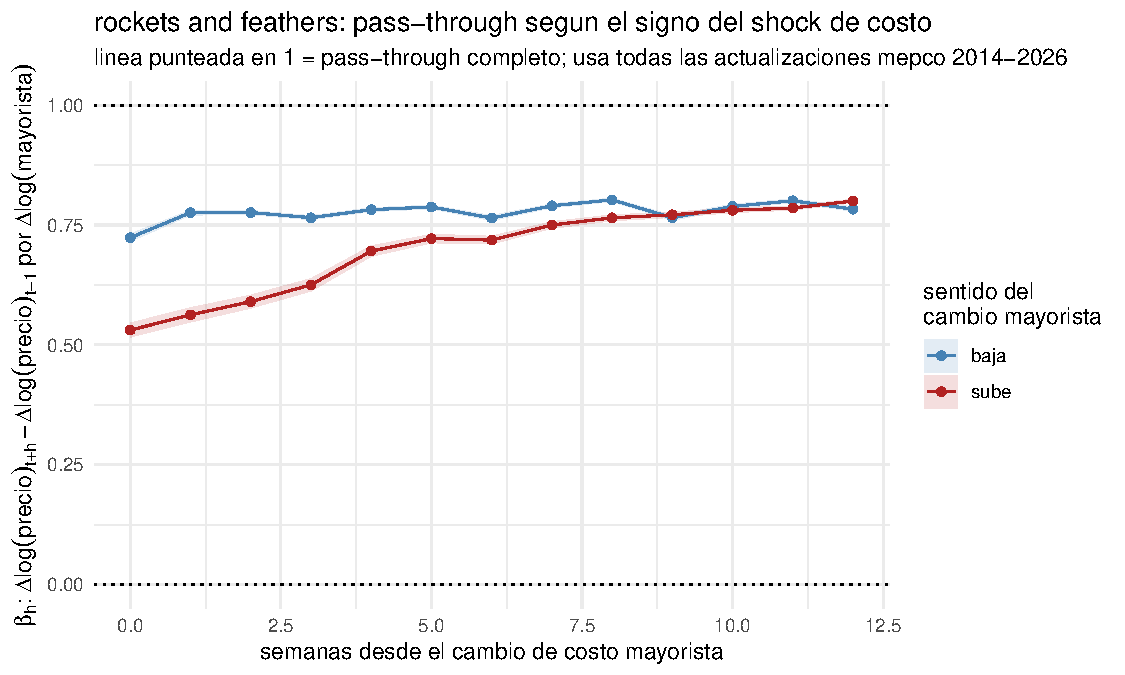
\includegraphics[width=0.85\textwidth]{../results/figures/rockets_feathers_irf.pdf}
\caption{Traspaso según el signo del shock de origen (partición muestral,
ecuación~\eqref{eq:rf_split}). Bandas de confianza al 95\% con errores
estándar agrupados por estación.}
\label{fig:rf_irf}
\end{figure}

\begin{figure}[htbp]
\centering
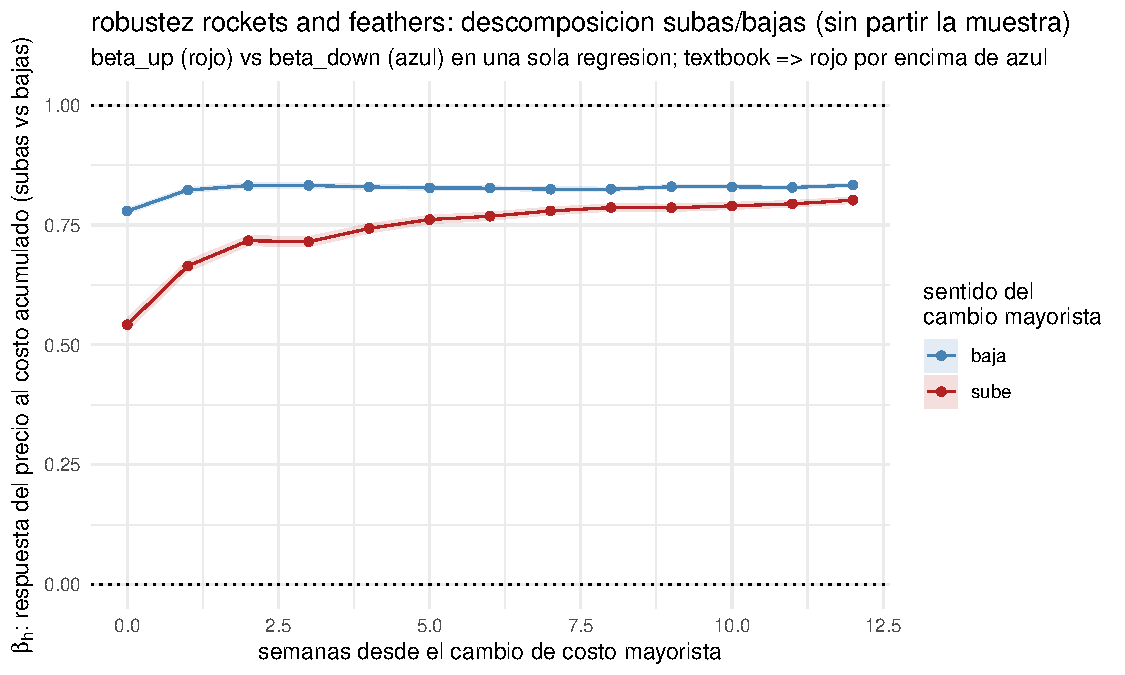
\includegraphics[width=0.85\textwidth]{../results/figures/rockets_feathers_robustness.pdf}
\caption{Descomposición de alzas y bajas en una sola regresión
(ecuación~\eqref{eq:rf_decomp}): $\beta_h^{+}$ y $\beta_h^{-}$ agregados.}
\label{fig:rf_rob}
\end{figure}

\begin{figure}[htbp]
\centering
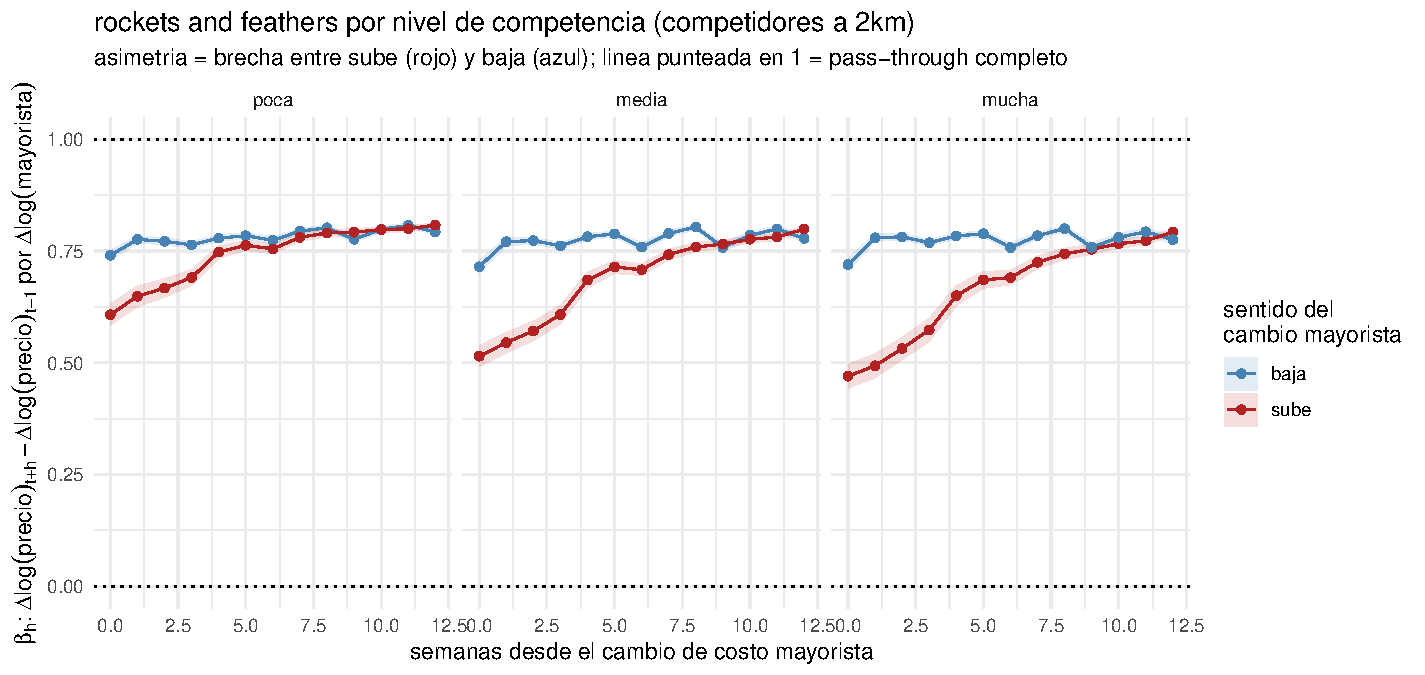
\includegraphics[width=\textwidth]{../results/figures/rockets_feathers_competencia.pdf}
\caption{Asimetría por nivel de competencia local (partición muestral por
signo dentro de cada tercil de competidores a 2 km).}
\label{fig:rf_comp}
\end{figure}

\begin{figure}[htbp]
\centering
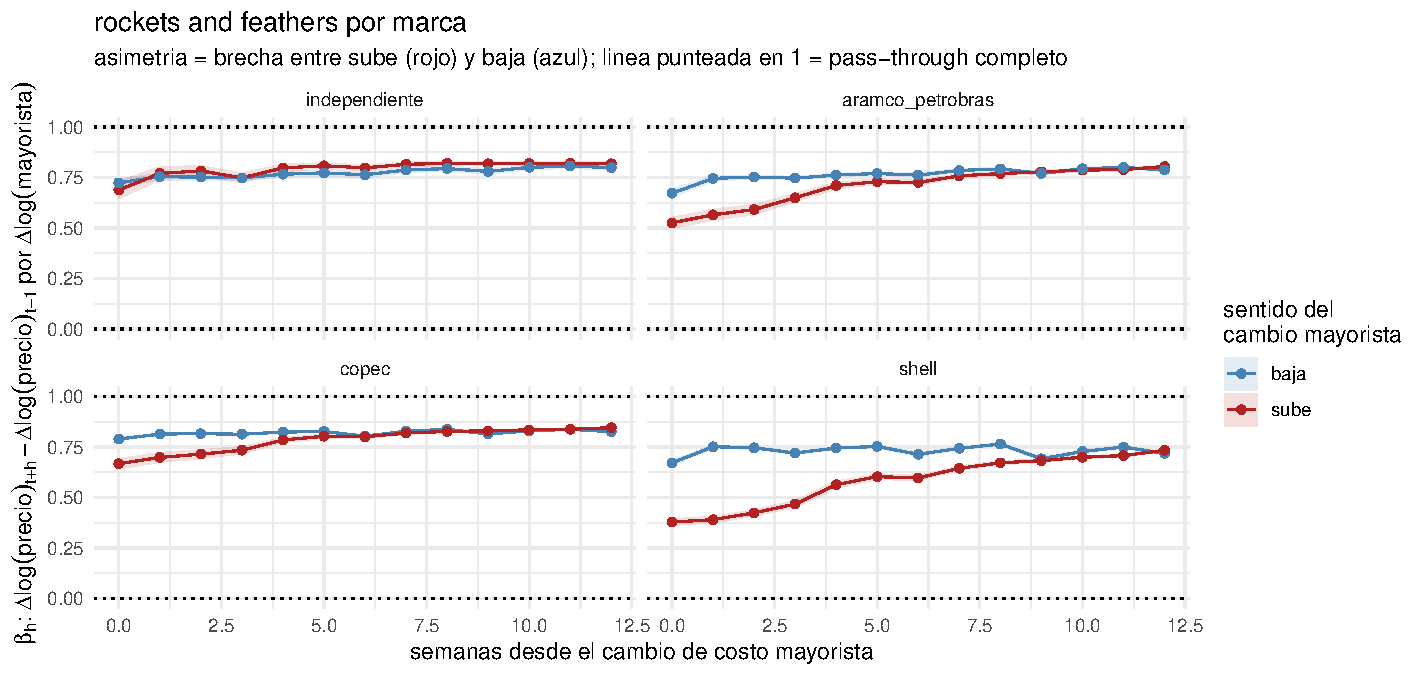
\includegraphics[width=\textwidth]{../results/figures/rockets_feathers_marca.pdf}
\caption{Asimetría por marca (partición muestral por signo dentro de cada
marca).}
\label{fig:rf_marca}
\end{figure}

\begin{figure}[htbp]
\centering
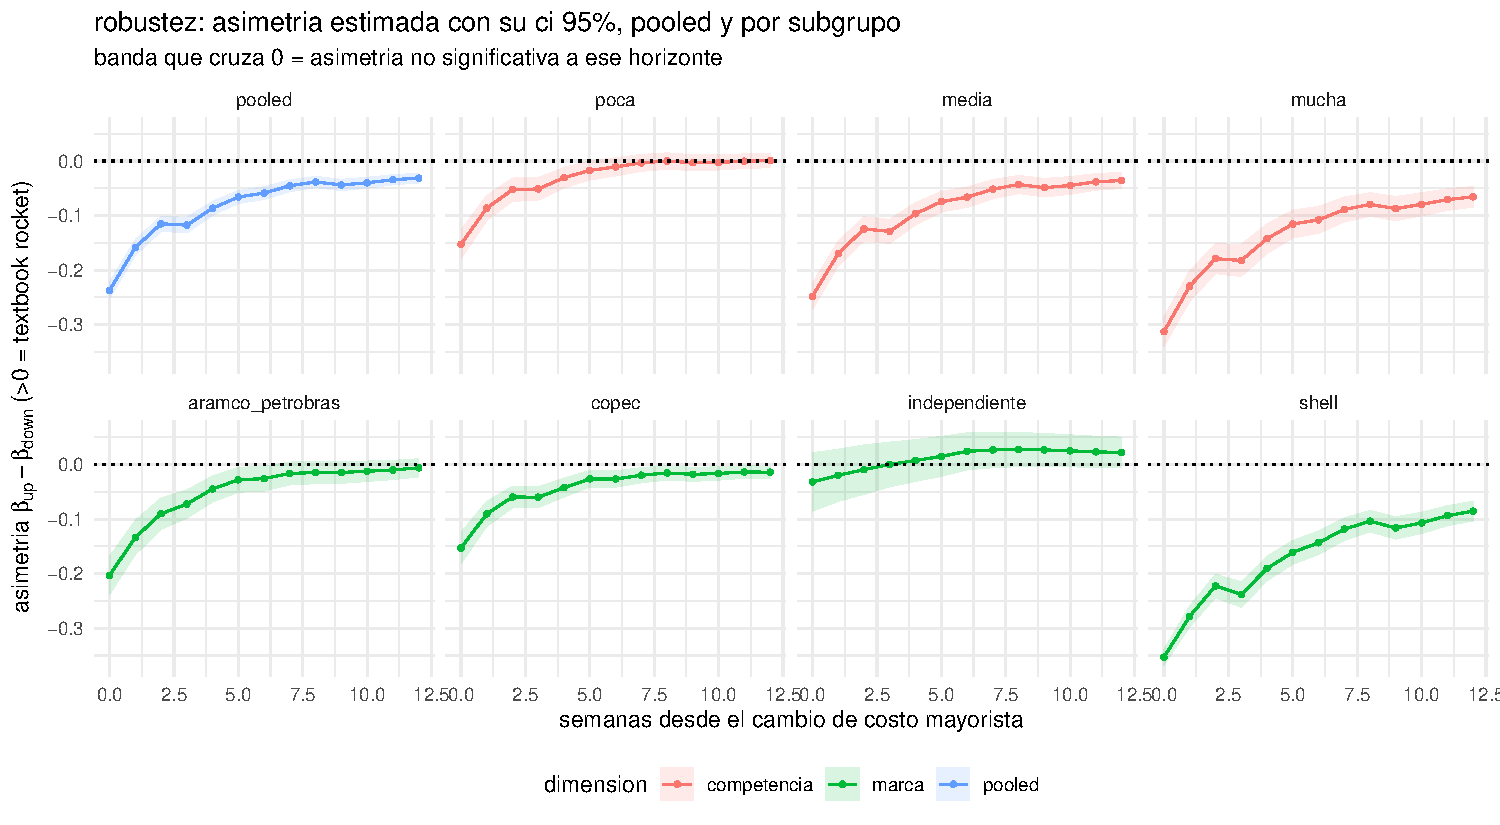
\includegraphics[width=\textwidth]{../results/figures/rockets_feathers_robustness_asym.pdf}
\caption{Asimetría $\beta_h^{+} - \beta_h^{-}$ con bandas de confianza al
95\%, agregada y por subgrupo (ecuación~\eqref{eq:rf_decomp}). Una banda que
cruza cero indica ausencia de asimetría significativa a ese horizonte.}
\label{fig:rf_asym}
\end{figure}

\section{Líderes y seguidores en la adopción del shock de marzo de 2026}
\label{sec:lider}

Esta sección baja a la escala intradiaria y pregunta cuándo, en fecha y
hora, cada distribuidor incorporó el shock de marzo de 2026 a sus precios de
venta. Para cada par estación-combustible se toma el primer cambio de precio
registrado entre el 26 de marzo y diez días después, medido en horas desde
las 00:00 del día del shock.\footnote{Cambios posteriores dentro de la
ventana pueden responder a otras causas y solo diluirían la medida de
adopción. La hora de reporte está disponible desde 2023.} El ejercicio es
descriptivo, un primer paso previo a cualquier modelo formal de liderazgo de
precios.

La marca temporal no es robusta como medida de decisión a nivel de estación.
Una fracción importante de los registros corresponde a cargas masivas desde
sistemas centrales, de modo que la hora observada mide cuándo el sistema del
distribuidor empujó la actualización y no una decisión estación por
estación.\footnote{Por ejemplo, 189 estaciones Shell comparten el segundo
idéntico de reporte (10:06:33 del 26 de marzo), 1.551 registros de esa red
caen dentro de una ventana de 20 segundos en torno a la 01:06 y el rango
intercuartílico de adopción de Shell es de 14 segundos.} Por eso la unidad
de análisis es el distribuidor o el grupo de estaciones, no la estación
individual. Un ejercicio líder-seguidor a nivel de estación estaría midiendo
infraestructura de carga de datos y no conducta de precios. Con esa
salvedad, las horas sí informan el patrón grueso entre tipos de operador,
madrugada frente a horario comercial y mismo día frente a días siguientes.

\subsection{Resultados}
\label{sec:lider_resultados}

La Tabla~\ref{tab:lider_dist} resume la adopción por distribuidor, para los
cinco con al menos 15 estaciones con cambio válido en la ventana. Las tres
grandes redes tenían el grueso de sus precios actualizados de madrugada. Las
medianas de Shell, Aramco-Petrobras y Copec corresponden a la 01:06, la
01:28 y las 02:02 del mismo 26 de marzo. Los operadores sin bandera y la
cadena regional HN ajustaron con mediana cercana a las once de la mañana y
colas que se extienden a los días siguientes.

\begin{table}[htbp]
\centering
\caption{Adopción del shock de marzo de 2026 por distribuidor (horas desde
las 00:00 del 26 de marzo hasta el primer cambio de precio).}
\label{tab:lider_dist}
\begin{tabular}{lcccc}
\toprule
Distribuidor & Estaciones & Mediana & P25 & P75 \\
\midrule
Shell             & 450 & 1,1  & 1,1 & 1,1 \\
Aramco-Petrobras  & 295 & 1,5  & 0,5 & 10,4 \\
Copec             & 688 & 2,0  & 0,6 & 8,6 \\
HN                & 16  & 10,4 & 9,2 & 35,4 \\
Sin bandera       & 68  & 10,9 & 8,8 & 17,9 \\
\bottomrule
\end{tabular}

\medskip
\begin{minipage}{0.85\textwidth}
\footnotesize
Nota: distribuidores con al menos 15 estaciones con un cambio de precio
válido en los diez días posteriores al shock. El rango intercuartílico de 14
segundos de Shell es la firma de una carga masiva centralizada.
\end{minipage}
\end{table}

Agrupando el total de la muestra en cadenas contra operadores chicos (sin
bandera o de estación única) quedan 4.505 pares estación-combustible en el
primer grupo y 278 en el segundo. La mediana de adopción es de 1,1 horas
para las cadenas contra 10,9 para los chicos, y el 94,9\% de las cadenas
había ajustado dentro de las primeras 24 horas contra el 82,4\% de los
chicos. La curva de adopción (Figura~\ref{fig:lider_curva}) muestra la forma
de la brecha. La de las cadenas es casi una escalera que salta en las
primeras horas de la madrugada, porque concentra cargas masivas, y la de los
chicos crece de forma gradual durante el primer y segundo día. El diagrama
de cajas (Figura~\ref{fig:lider_boxplot}) agrega que Copec y
Aramco-Petrobras, a diferencia de Shell, combinan un bloque de madrugada con
una cola que ajusta durante el día (P75 de 8,6 y 10,4 horas), lo que sugiere
actualizaciones escalonadas por zona.

Las regresiones de las Tablas~\ref{tab:lider_reg} y~\ref{tab:lider_comp}
cuantifican la brecha con errores estándar agrupados por distribuidor,
porque las estaciones de una misma red no ajustan de manera independiente.
Pertenecer a una cadena reduce el tiempo de adopción a cerca de un cuarto
(coeficiente de $-1{,}38$ en $\log(\text{horas}+1)$) y la velocidad escala
con el tamaño de la red, pues duplicar el número de estaciones del
distribuidor reduce el tiempo en torno al 16\%. La competencia local no
predice la velocidad intradiaria. Ni el conteo de rivales a 2 km ni la
intensidad continua tienen coeficientes distinguibles de cero, con o sin
control por tamaño de red. Esto replica en horas lo encontrado a frecuencia
semanal en la Sección~\ref{sec:lp_evento}.

\begin{table}[htbp]
\centering
\caption{Velocidad de adopción: cadena contra operador chico y tamaño de
red.}
\label{tab:lider_reg}

\begingroup
\centering
\begin{tabular}{lcc}
   \tabularnewline \midrule \midrule
   Dependent Variable: & \multicolumn{2}{c}{log(hours\_since\_shock+1)}\\
   Model:                                & (1)            & (2)\\  
   \midrule
   \emph{Variables}\\
   Constant                              & 2.737$^{***}$  & 2.989$^{***}$\\   
                                         & (0.0684)       & (0.2173)\\   
   is\_franchise\_preTRUE                & -1.380$^{***}$ &   \\   
                                         & (0.1512)       &   \\   
   log(distributor\_n\_stations\_pre)    &                & -0.2495$^{***}$\\   
                                         &                & (0.0398)\\   
   competitors\_2km\_pre                 &                & -0.0141\\   
                                         &                & (0.0118)\\   
   \midrule
   \emph{Fit statistics}\\
   Observations                          & 4,783          & 4,783\\  
   R$^2$                                 & 0.07944        & 0.11154\\  
   Adjusted R$^2$                        & 0.07925        & 0.11117\\  
   \midrule \midrule
   \multicolumn{3}{l}{\emph{Clustered (distributor) standard-errors in parentheses}}\\
   \multicolumn{3}{l}{\emph{Signif. Codes: ***: 0.01, **: 0.05, *: 0.1}}\\
\end{tabular}
\par\endgroup




\medskip
\begin{minipage}{0.85\textwidth}
\footnotesize
Nota: variable dependiente $\log(\text{horas desde el shock} + 1)$ del
primer cambio de precio del par estación-combustible.
\texttt{is\_franchise\_pre} indica cadena (distribuidor con marca y más de
una estación), \texttt{distributor\_n\_stations\_pre} es el número de
estaciones del distribuidor y \texttt{competitors\_2km\_pre} el número de
rivales a 2 km, todos fijados antes del shock. Errores estándar agrupados
por distribuidor.
\end{minipage}
\end{table}

\begin{table}[htbp]
\centering
\caption{Velocidad de adopción y competencia local (intensidad continua).}
\label{tab:lider_comp}

\begingroup
\centering
\begin{tabular}{lcc}
   \tabularnewline \midrule \midrule
   Dependent Variable: & \multicolumn{2}{c}{log(hours\_since\_shock+1)}\\
   Model:                                & (1)           & (2)\\  
   \midrule
   \emph{Variables}\\
   Constant                              & 1.542$^{***}$ & 2.982$^{***}$\\   
                                         & (0.1735)      & (0.2215)\\   
   competition\_intensity\_pre           & -0.0071       & -0.0045\\   
                                         & (0.0063)      & (0.0051)\\   
   log(distributor\_n\_stations\_pre)    &               & -0.2493$^{***}$\\   
                                         &               & (0.0394)\\   
   \midrule
   \emph{Fit statistics}\\
   Observations                          & 4,783         & 4,783\\  
   R$^2$                                 & 0.00751       & 0.11137\\  
   Adjusted R$^2$                        & 0.00730       & 0.11100\\  
   \midrule \midrule
   \multicolumn{3}{l}{\emph{Clustered (distributor) standard-errors in parentheses}}\\
   \multicolumn{3}{l}{\emph{Signif. Codes: ***: 0.01, **: 0.05, *: 0.1}}\\
\end{tabular}
\par\endgroup




\medskip
\begin{minipage}{0.85\textwidth}
\footnotesize
Nota: \texttt{competition\_intensity\_pre} es la medida continua de
competencia ponderada por el inverso de la distancia
(ecuación~\eqref{eq:intensity}), fijada antes del shock. Errores estándar
agrupados por distribuidor.
\end{minipage}
\end{table}

La interpretación económica, con la cautela que impone la calidad de la
marca temporal, es coherente con los dos tipos de operador. Las cadenas
actualizan según un plan, con precios cargados de forma centralizada en la
madrugada misma en que el nuevo mayorista entra en vigencia. Las
independientes ajustan en base a los precios de mercado, durante el horario
comercial y con uno o dos días de rezago, tiempo consistente con observar
primero los precios de los rivales de cadena y responder después. Bajo esa
lectura, el liderazgo de precios frente a un shock de costo público lo
ejercen las redes grandes y las independientes actúan como seguidoras en la
escala intradiaria. Esto no contradice su traspaso alto y rápido a
frecuencia semanal, porque uno o dos días de rezago son invisibles en la
grilla semanal, donde lo que las distingue es cuánto traspasan y no la hora
exacta en que lo hacen.

\begin{figure}[htbp]
\centering
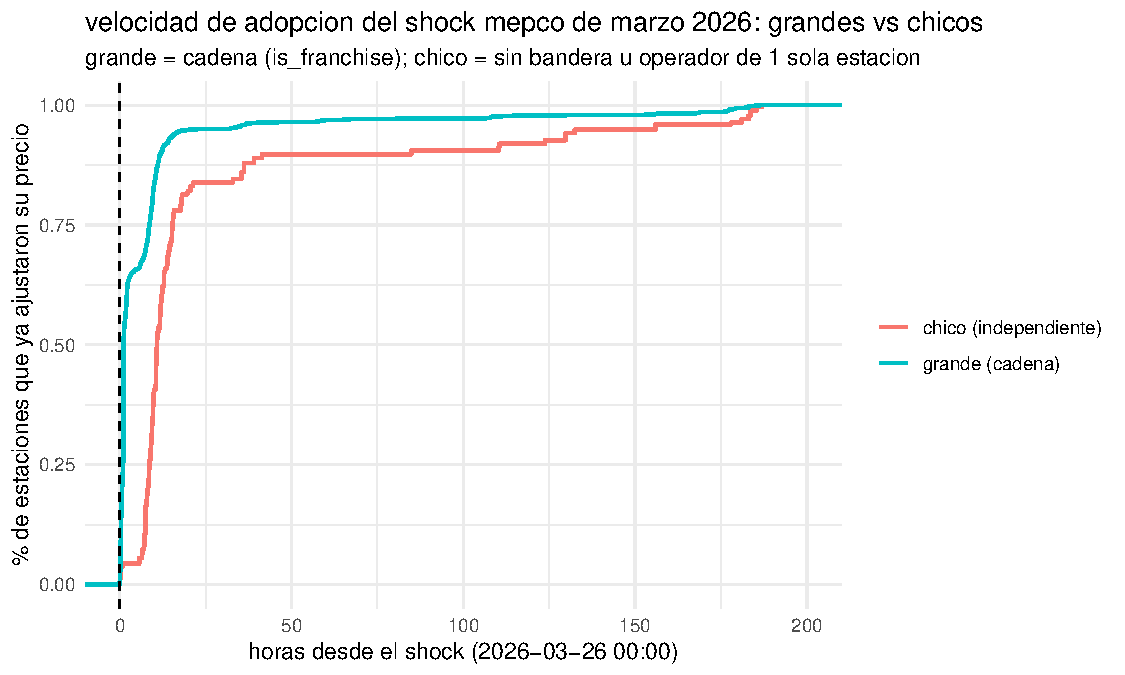
\includegraphics[width=0.85\textwidth]{../results/figures/leader_follower_adoption_curve.pdf}
\caption{Curva de adopción del shock de marzo de 2026: proporción acumulada
de pares estación-combustible que ya ajustaron su precio, por grupo.}
\label{fig:lider_curva}
\end{figure}

\begin{figure}[htbp]
\centering
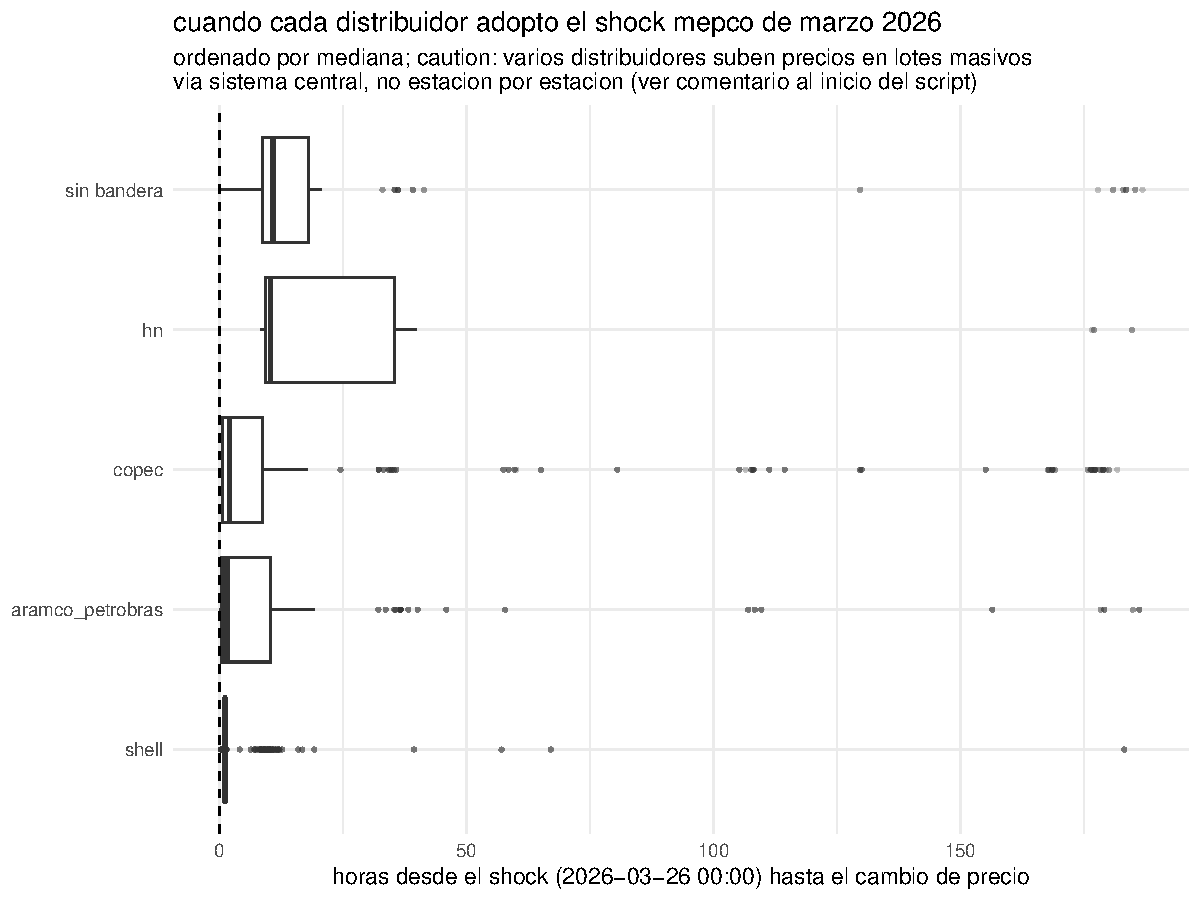
\includegraphics[width=0.85\textwidth]{../results/figures/leader_follower_boxplot.pdf}
\caption{Distribución de la hora de adopción por distribuidor (ordenados por
mediana). Las cajas comprimidas reflejan cargas masivas centralizadas.}
\label{fig:lider_boxplot}
\end{figure}

\end{document}
